\documentclass[twoside]{book}

% Packages required by doxygen
\usepackage{fixltx2e}
\usepackage{calc}
\usepackage{doxygen}
\usepackage[export]{adjustbox} % also loads graphicx
\usepackage{graphicx}
\usepackage[utf8]{inputenc}
\usepackage{makeidx}
\usepackage{multicol}
\usepackage{multirow}
\PassOptionsToPackage{warn}{textcomp}
\usepackage{textcomp}
\usepackage[nointegrals]{wasysym}
\usepackage[table]{xcolor}

% NLS support packages
\usepackage[T2A]{fontenc}
\usepackage[russian]{babel}

% Font selection
\usepackage[T1]{fontenc}
\usepackage[scaled=.90]{helvet}
\usepackage{courier}
\usepackage{amssymb}
\usepackage{sectsty}
\renewcommand{\familydefault}{\sfdefault}
\allsectionsfont{%
  \fontseries{bc}\selectfont%
  \color{darkgray}%
}
\renewcommand{\DoxyLabelFont}{%
  \fontseries{bc}\selectfont%
  \color{darkgray}%
}
\newcommand{\+}{\discretionary{\mbox{\scriptsize$\hookleftarrow$}}{}{}}

% Page & text layout
\usepackage{geometry}
\geometry{%
  a4paper,%
  top=2.5cm,%
  bottom=2.5cm,%
  left=2.5cm,%
  right=2.5cm%
}
\tolerance=750
\hfuzz=15pt
\hbadness=750
\setlength{\emergencystretch}{15pt}
\setlength{\parindent}{0cm}
\setlength{\parskip}{3ex plus 2ex minus 2ex}
\makeatletter
\renewcommand{\paragraph}{%
  \@startsection{paragraph}{4}{0ex}{-1.0ex}{1.0ex}{%
    \normalfont\normalsize\bfseries\SS@parafont%
  }%
}
\renewcommand{\subparagraph}{%
  \@startsection{subparagraph}{5}{0ex}{-1.0ex}{1.0ex}{%
    \normalfont\normalsize\bfseries\SS@subparafont%
  }%
}
\makeatother

% Headers & footers
\usepackage{fancyhdr}
\pagestyle{fancyplain}
\fancyhead[LE]{\fancyplain{}{\bfseries\thepage}}
\fancyhead[CE]{\fancyplain{}{}}
\fancyhead[RE]{\fancyplain{}{\bfseries\leftmark}}
\fancyhead[LO]{\fancyplain{}{\bfseries\rightmark}}
\fancyhead[CO]{\fancyplain{}{}}
\fancyhead[RO]{\fancyplain{}{\bfseries\thepage}}
\fancyfoot[LE]{\fancyplain{}{}}
\fancyfoot[CE]{\fancyplain{}{}}
\fancyfoot[RE]{\fancyplain{}{\bfseries\scriptsize Создано системой Doxygen }}
\fancyfoot[LO]{\fancyplain{}{\bfseries\scriptsize Создано системой Doxygen }}
\fancyfoot[CO]{\fancyplain{}{}}
\fancyfoot[RO]{\fancyplain{}{}}
\renewcommand{\footrulewidth}{0.4pt}
\renewcommand{\chaptermark}[1]{%
  \markboth{#1}{}%
}
\renewcommand{\sectionmark}[1]{%
  \markright{\thesection\ #1}%
}

% Indices & bibliography
\usepackage{natbib}
\usepackage[titles]{tocloft}
\setcounter{tocdepth}{3}
\setcounter{secnumdepth}{5}
\makeindex

% Hyperlinks (required, but should be loaded last)
\usepackage{ifpdf}
\ifpdf
  \usepackage[pdftex,pagebackref=true]{hyperref}
\else
  \usepackage[ps2pdf,pagebackref=true]{hyperref}
\fi
\hypersetup{%
  colorlinks=true,%
  linkcolor=blue,%
  citecolor=blue,%
  unicode%
}

% Custom commands
\newcommand{\clearemptydoublepage}{%
  \newpage{\pagestyle{empty}\cleardoublepage}%
}

\usepackage{caption}
\captionsetup{labelsep=space,justification=centering,font={bf},singlelinecheck=off,skip=4pt,position=top}

%===== C O N T E N T S =====

\begin{document}

% Titlepage & ToC
\hypersetup{pageanchor=false,
             bookmarksnumbered=true,
             pdfencoding=unicode
            }
\pagenumbering{alph}
\begin{titlepage}
\vspace*{7cm}
\begin{center}%
{\Large Nedo\+Chat \\[1ex]\large 1.\+0.\+0 }\\
\vspace*{1cm}
{\large Создано системой Doxygen 1.8.14}\\
\end{center}
\end{titlepage}
\clearemptydoublepage
\pagenumbering{roman}
\tableofcontents
\clearemptydoublepage
\pagenumbering{arabic}
\hypersetup{pageanchor=true}

%--- Begin generated contents ---
\chapter{Алфавитный указатель пространств имен}
\section{Пакеты}
Полный список документированных пакетов.\begin{DoxyCompactList}
\item\contentsline{section}{\mbox{\hyperlink{namespacecom}{com}} }{\pageref{namespacecom}}{}
\item\contentsline{section}{\mbox{\hyperlink{namespacecom_1_1example}{com.\+example}} }{\pageref{namespacecom_1_1example}}{}
\item\contentsline{section}{\mbox{\hyperlink{namespacecom_1_1example_1_1firebasechat}{com.\+example.\+firebasechat}} }{\pageref{namespacecom_1_1example_1_1firebasechat}}{}
\end{DoxyCompactList}

\chapter{Иерархический список классов}
\section{Иерархия классов}
Иерархия классов.\begin{DoxyCompactList}
\item \contentsline{section}{com.\+example.\+firebasechat.\+Message}{\pageref{classcom_1_1example_1_1firebasechat_1_1_message}}{}
\item On\+Click\+Listener\begin{DoxyCompactList}
\item \contentsline{section}{com.\+example.\+firebasechat.\+Main\+Activity}{\pageref{classcom_1_1example_1_1firebasechat_1_1_main_activity}}{}
\end{DoxyCompactList}
\item \contentsline{section}{com.\+example.\+firebasechat.\+User}{\pageref{classcom_1_1example_1_1firebasechat_1_1_user}}{}
\item View\+Holder\begin{DoxyCompactList}
\item \contentsline{section}{com.\+example.\+firebasechat.\+View\+Holder}{\pageref{classcom_1_1example_1_1firebasechat_1_1_view_holder}}{}
\end{DoxyCompactList}
\item App\+Compat\+Activity\begin{DoxyCompactList}
\item \contentsline{section}{com.\+example.\+firebasechat.\+Authors}{\pageref{classcom_1_1example_1_1firebasechat_1_1_authors}}{}
\item \contentsline{section}{com.\+example.\+firebasechat.\+Chat\+Room}{\pageref{classcom_1_1example_1_1firebasechat_1_1_chat_room}}{}
\item \contentsline{section}{com.\+example.\+firebasechat.\+Main\+Activity}{\pageref{classcom_1_1example_1_1firebasechat_1_1_main_activity}}{}
\item \contentsline{section}{com.\+example.\+firebasechat.\+Splash\+Activity}{\pageref{classcom_1_1example_1_1firebasechat_1_1_splash_activity}}{}
\end{DoxyCompactList}
\item Async\+Task\begin{DoxyCompactList}
\item \contentsline{section}{com.\+example.\+firebasechat.\+Main\+Activity.\+Key\+\_\+\+Thread}{\pageref{classcom_1_1example_1_1firebasechat_1_1_main_activity_1_1_key___thread}}{}
\end{DoxyCompactList}
\end{DoxyCompactList}

\chapter{Алфавитный указатель классов}
\section{Классы}
Классы с их кратким описанием.\begin{DoxyCompactList}
\item\contentsline{section}{\mbox{\hyperlink{classcom_1_1example_1_1firebasechat_1_1_authors}{com.\+example.\+firebasechat.\+Authors}} \\*Класс для отображения страницы с информацией о создателях }{\pageref{classcom_1_1example_1_1firebasechat_1_1_authors}}{}
\item\contentsline{section}{\mbox{\hyperlink{classcom_1_1example_1_1firebasechat_1_1_chat_room}{com.\+example.\+firebasechat.\+Chat\+Room}} \\*Данное Activity представляет собой комнату обмена зашифрованными сообщениями }{\pageref{classcom_1_1example_1_1firebasechat_1_1_chat_room}}{}
\item\contentsline{section}{\mbox{\hyperlink{classcom_1_1example_1_1firebasechat_1_1_main_activity_1_1_key___thread}{com.\+example.\+firebasechat.\+Main\+Activity.\+Key\+\_\+\+Thread}} \\*Поток для обработки генерации ключей }{\pageref{classcom_1_1example_1_1firebasechat_1_1_main_activity_1_1_key___thread}}{}
\item\contentsline{section}{\mbox{\hyperlink{classcom_1_1example_1_1firebasechat_1_1_main_activity}{com.\+example.\+firebasechat.\+Main\+Activity}} \\*Activity регистрации и авторизации пользователей }{\pageref{classcom_1_1example_1_1firebasechat_1_1_main_activity}}{}
\item\contentsline{section}{\mbox{\hyperlink{classcom_1_1example_1_1firebasechat_1_1_message}{com.\+example.\+firebasechat.\+Message}} \\*Класс сообщений пользователей }{\pageref{classcom_1_1example_1_1firebasechat_1_1_message}}{}
\item\contentsline{section}{\mbox{\hyperlink{classcom_1_1example_1_1firebasechat_1_1_splash_activity}{com.\+example.\+firebasechat.\+Splash\+Activity}} \\*Заставка приложения }{\pageref{classcom_1_1example_1_1firebasechat_1_1_splash_activity}}{}
\item\contentsline{section}{\mbox{\hyperlink{classcom_1_1example_1_1firebasechat_1_1_user}{com.\+example.\+firebasechat.\+User}} \\*Класс пользователя }{\pageref{classcom_1_1example_1_1firebasechat_1_1_user}}{}
\item\contentsline{section}{\mbox{\hyperlink{classcom_1_1example_1_1firebasechat_1_1_view_holder}{com.\+example.\+firebasechat.\+View\+Holder}} \\*Класс holder отображения сообщений в Recycler\+View }{\pageref{classcom_1_1example_1_1firebasechat_1_1_view_holder}}{}
\end{DoxyCompactList}

\chapter{Список файлов}
\section{Файлы}
Полный список файлов.\begin{DoxyCompactList}
\item\contentsline{section}{C\+:/\+Games/\+Back\+Up/\+Fire\+Basechat/app/src/main/java/com/example/firebasechat/\mbox{\hyperlink{_authors_8java}{Authors.\+java}} }{\pageref{_authors_8java}}{}
\item\contentsline{section}{C\+:/\+Games/\+Back\+Up/\+Fire\+Basechat/app/src/main/java/com/example/firebasechat/\mbox{\hyperlink{_chat_room_8java}{Chat\+Room.\+java}} }{\pageref{_chat_room_8java}}{}
\item\contentsline{section}{C\+:/\+Games/\+Back\+Up/\+Fire\+Basechat/app/src/main/java/com/example/firebasechat/\mbox{\hyperlink{_main_activity_8java}{Main\+Activity.\+java}} }{\pageref{_main_activity_8java}}{}
\item\contentsline{section}{C\+:/\+Games/\+Back\+Up/\+Fire\+Basechat/app/src/main/java/com/example/firebasechat/\mbox{\hyperlink{_message_8java}{Message.\+java}} }{\pageref{_message_8java}}{}
\item\contentsline{section}{C\+:/\+Games/\+Back\+Up/\+Fire\+Basechat/app/src/main/java/com/example/firebasechat/\mbox{\hyperlink{_splash_activity_8java}{Splash\+Activity.\+java}} }{\pageref{_splash_activity_8java}}{}
\item\contentsline{section}{C\+:/\+Games/\+Back\+Up/\+Fire\+Basechat/app/src/main/java/com/example/firebasechat/\mbox{\hyperlink{_user_8java}{User.\+java}} }{\pageref{_user_8java}}{}
\item\contentsline{section}{C\+:/\+Games/\+Back\+Up/\+Fire\+Basechat/app/src/main/java/com/example/firebasechat/\mbox{\hyperlink{_view_holder_8java}{View\+Holder.\+java}} }{\pageref{_view_holder_8java}}{}
\end{DoxyCompactList}

\chapter{Пространства имен}
\hypertarget{namespacecom}{}\section{Пакет com}
\label{namespacecom}\index{com@{com}}
\subsection*{Пакеты}
\begin{DoxyCompactItemize}
\item 
package \mbox{\hyperlink{namespacecom_1_1example}{example}}
\end{DoxyCompactItemize}

\hypertarget{namespacecom_1_1example}{}\section{Пакет com.\+example}
\label{namespacecom_1_1example}\index{com.\+example@{com.\+example}}
\subsection*{Пакеты}
\begin{DoxyCompactItemize}
\item 
package \mbox{\hyperlink{namespacecom_1_1example_1_1firebasechat}{firebasechat}}
\end{DoxyCompactItemize}

\hypertarget{namespacecom_1_1example_1_1firebasechat}{}\section{Пакет com.\+example.\+firebasechat}
\label{namespacecom_1_1example_1_1firebasechat}\index{com.\+example.\+firebasechat@{com.\+example.\+firebasechat}}
\subsection*{Классы}
\begin{DoxyCompactItemize}
\item 
class \mbox{\hyperlink{classcom_1_1example_1_1firebasechat_1_1_authors}{Authors}}
\begin{DoxyCompactList}\small\item\em Класс для отображения страницы с информацией о создателях \end{DoxyCompactList}\item 
class \mbox{\hyperlink{classcom_1_1example_1_1firebasechat_1_1_chat_room}{Chat\+Room}}
\begin{DoxyCompactList}\small\item\em Данное Activity представляет собой комнату обмена зашифрованными сообщениями \end{DoxyCompactList}\item 
class \mbox{\hyperlink{classcom_1_1example_1_1firebasechat_1_1_main_activity}{Main\+Activity}}
\begin{DoxyCompactList}\small\item\em Activity регистрации и авторизации пользователей \end{DoxyCompactList}\item 
class \mbox{\hyperlink{classcom_1_1example_1_1firebasechat_1_1_message}{Message}}
\begin{DoxyCompactList}\small\item\em Класс сообщений пользователей \end{DoxyCompactList}\item 
class \mbox{\hyperlink{classcom_1_1example_1_1firebasechat_1_1_splash_activity}{Splash\+Activity}}
\begin{DoxyCompactList}\small\item\em Заставка приложения \end{DoxyCompactList}\item 
class \mbox{\hyperlink{classcom_1_1example_1_1firebasechat_1_1_user}{User}}
\begin{DoxyCompactList}\small\item\em Класс пользователя \end{DoxyCompactList}\item 
class \mbox{\hyperlink{classcom_1_1example_1_1firebasechat_1_1_view_holder}{View\+Holder}}
\begin{DoxyCompactList}\small\item\em Класс holder отображения сообщений в Recycler\+View. \end{DoxyCompactList}\end{DoxyCompactItemize}

\chapter{Классы}
\hypertarget{classcom_1_1example_1_1firebasechat_1_1_authors}{}\section{Класс com.\+example.\+firebasechat.\+Authors}
\label{classcom_1_1example_1_1firebasechat_1_1_authors}\index{com.\+example.\+firebasechat.\+Authors@{com.\+example.\+firebasechat.\+Authors}}


Класс для отображения страницы с информацией о создателях  


Граф наследования\+:com.\+example.\+firebasechat.\+Authors\+:\begin{figure}[H]
\begin{center}
\leavevmode
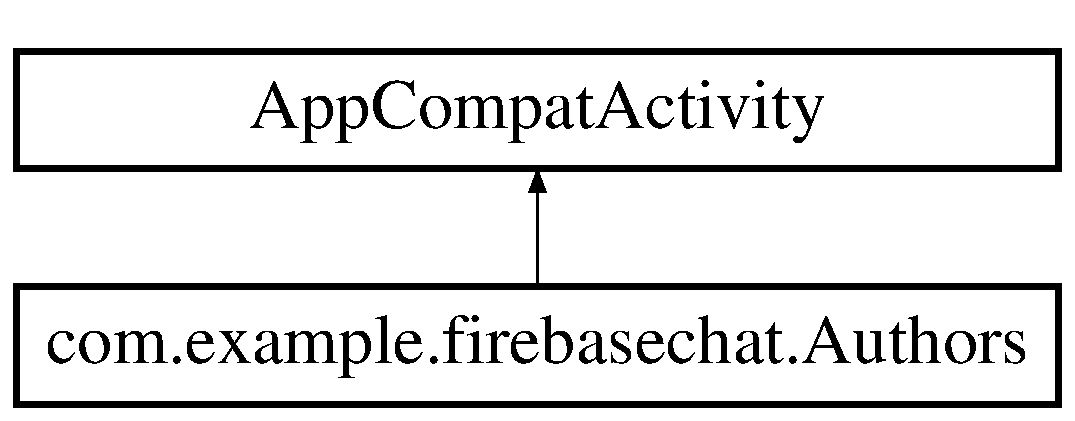
\includegraphics[height=2.000000cm]{classcom_1_1example_1_1firebasechat_1_1_authors}
\end{center}
\end{figure}
\subsection*{Защищенные члены}
\begin{DoxyCompactItemize}
\item 
void \mbox{\hyperlink{classcom_1_1example_1_1firebasechat_1_1_authors_a9482fe36b1cabddda1532d2c5633daa3}{on\+Create}} (Bundle saved\+Instance\+State)
\begin{DoxyCompactList}\small\item\em Создание activity \mbox{\hyperlink{classcom_1_1example_1_1firebasechat_1_1_authors}{Authors}}. \end{DoxyCompactList}\end{DoxyCompactItemize}


\subsection{Подробное описание}
Класс для отображения страницы с информацией о создателях 

См. определение в файле Authors.\+java строка 13



\subsection{Методы}
\mbox{\Hypertarget{classcom_1_1example_1_1firebasechat_1_1_authors_a9482fe36b1cabddda1532d2c5633daa3}\label{classcom_1_1example_1_1firebasechat_1_1_authors_a9482fe36b1cabddda1532d2c5633daa3}} 
\index{com\+::example\+::firebasechat\+::\+Authors@{com\+::example\+::firebasechat\+::\+Authors}!on\+Create@{on\+Create}}
\index{on\+Create@{on\+Create}!com\+::example\+::firebasechat\+::\+Authors@{com\+::example\+::firebasechat\+::\+Authors}}
\subsubsection{\texorpdfstring{on\+Create()}{onCreate()}}
{\footnotesize\ttfamily void com.\+example.\+firebasechat.\+Authors.\+on\+Create (\begin{DoxyParamCaption}\item[{Bundle}]{saved\+Instance\+State }\end{DoxyParamCaption})\hspace{0.3cm}{\ttfamily [protected]}}



Создание activity \mbox{\hyperlink{classcom_1_1example_1_1firebasechat_1_1_authors}{Authors}}. 


\begin{DoxyParams}{Аргументы}
{\em saved\+Instance\+State} & \\
\hline
\end{DoxyParams}


См. определение в файле Authors.\+java строка 22



Объявления и описания членов класса находятся в файле\+:\begin{DoxyCompactItemize}
\item 
C\+:/\+Games/\+Back\+Up/\+Fire\+Basechat/app/src/main/java/com/example/firebasechat/\mbox{\hyperlink{_authors_8java}{Authors.\+java}}\end{DoxyCompactItemize}

\hypertarget{classcom_1_1example_1_1firebasechat_1_1_chat_room}{}\section{Класс com.\+example.\+firebasechat.\+Chat\+Room}
\label{classcom_1_1example_1_1firebasechat_1_1_chat_room}\index{com.\+example.\+firebasechat.\+Chat\+Room@{com.\+example.\+firebasechat.\+Chat\+Room}}


Данное Activity представляет собой комнату обмена зашифрованными сообщениями  


Граф наследования\+:com.\+example.\+firebasechat.\+Chat\+Room\+:\begin{figure}[H]
\begin{center}
\leavevmode
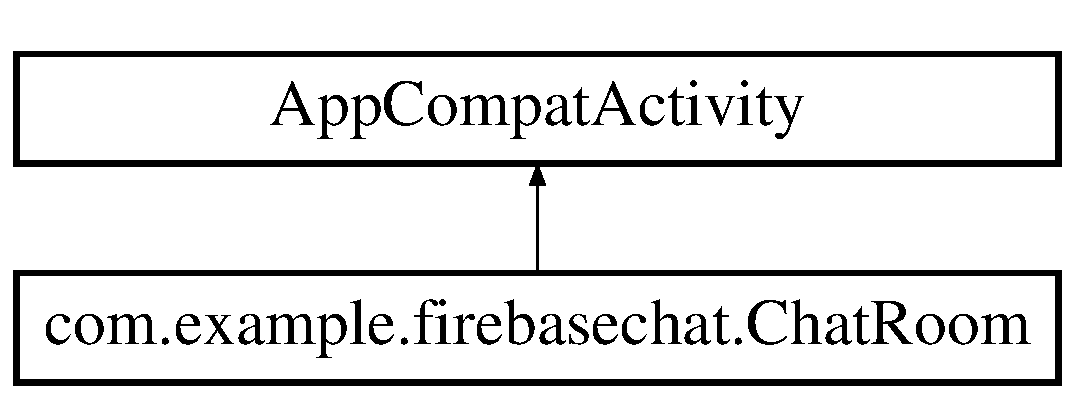
\includegraphics[height=2.000000cm]{classcom_1_1example_1_1firebasechat_1_1_chat_room}
\end{center}
\end{figure}
\subsection*{Открытые члены}
\begin{DoxyCompactItemize}
\item 
void \mbox{\hyperlink{classcom_1_1example_1_1firebasechat_1_1_chat_room_a4523f252ff4e59d283df68e2844d8019}{display\+Chat}} ()
\begin{DoxyCompactList}\small\item\em Функция отображения сообщений \end{DoxyCompactList}\item 
void \mbox{\hyperlink{classcom_1_1example_1_1firebasechat_1_1_chat_room_a581058422cc44701b83f7c2a298406a9}{get\+\_\+keys}} ()
\begin{DoxyCompactList}\small\item\em Данная функция предназначена для получения ключей \end{DoxyCompactList}\item 
void \mbox{\hyperlink{classcom_1_1example_1_1firebasechat_1_1_chat_room_a2772aea181483bc52c5fdffcf7fb9f79}{Admin\+\_\+actrivity}} ()
\begin{DoxyCompactList}\small\item\em Данная функция предназначена для обработки публичных ключей администатором \end{DoxyCompactList}\item 
boolean \mbox{\hyperlink{classcom_1_1example_1_1firebasechat_1_1_chat_room_a2c0ed8faa3bb7d8d5ac7959292c113fa}{on\+Create\+Options\+Menu}} (Menu menu)
\begin{DoxyCompactList}\small\item\em Функция создания кнопки выхода \end{DoxyCompactList}\item 
boolean \mbox{\hyperlink{classcom_1_1example_1_1firebasechat_1_1_chat_room_a278ca3b8374bddc73823cf42eeb62ba2}{on\+Options\+Item\+Selected}} (Menu\+Item item)
\begin{DoxyCompactList}\small\item\em Обработка нажатия на кнопку выхода \end{DoxyCompactList}\end{DoxyCompactItemize}
\subsection*{Открытые атрибуты}
\begin{DoxyCompactItemize}
\item 
Firebase\+List\+Adapter$<$ \mbox{\hyperlink{classcom_1_1example_1_1firebasechat_1_1_message}{Message}} $>$ \mbox{\hyperlink{classcom_1_1example_1_1firebasechat_1_1_chat_room_aea339a52dcfcefb9f710a47548f37fed}{adapter}}
\begin{DoxyCompactList}\small\item\em Адаптер для отображения сообщений с сервера \end{DoxyCompactList}\item 
Database\+Reference \mbox{\hyperlink{classcom_1_1example_1_1firebasechat_1_1_chat_room_af6807d5446ac002a074f0ad11724ce71}{Admen}} = Firebase\+Database.\+get\+Instance().get\+Reference(\char`\"{}Admen\char`\"{})
\begin{DoxyCompactList}\small\item\em База данных с обработанными Администратором публичными ключами пользователей \end{DoxyCompactList}\item 
Database\+Reference \mbox{\hyperlink{classcom_1_1example_1_1firebasechat_1_1_chat_room_adb882b49c6dbcbe1508d090eb2507505}{messages}} = Firebase\+Database.\+get\+Instance().get\+Reference(\char`\"{}messages\char`\"{})
\begin{DoxyCompactList}\small\item\em База данных с сообщениям пользователей \end{DoxyCompactList}\item 
Database\+Reference \mbox{\hyperlink{classcom_1_1example_1_1firebasechat_1_1_chat_room_ad3a0dbe421eb87403be4582e54eac253}{pkeys}} = Firebase\+Database.\+get\+Instance().get\+Reference(\char`\"{}Public\+\_\+\+Key\char`\"{})
\begin{DoxyCompactList}\small\item\em Базад данных публичных ключей \end{DoxyCompactList}\end{DoxyCompactItemize}
\subsection*{Статические открытые данные}
\begin{DoxyCompactItemize}
\item 
static int \mbox{\hyperlink{classcom_1_1example_1_1firebasechat_1_1_chat_room_a16b9729a48a21196941e042b2768cb26}{M\+A\+X\+\_\+\+M\+E\+S\+S\+A\+G\+E\+\_\+\+L\+E\+N\+G\+TH}} = 300
\begin{DoxyCompactList}\small\item\em Максимальная длина сообщения \end{DoxyCompactList}\end{DoxyCompactItemize}
\subsection*{Защищенные члены}
\begin{DoxyCompactItemize}
\item 
void \mbox{\hyperlink{classcom_1_1example_1_1firebasechat_1_1_chat_room_a5eb5c76ba6bdb4aa636bf1bd26364a02}{on\+Create}} (Bundle saved\+Instance\+State)
\end{DoxyCompactItemize}


\subsection{Подробное описание}
Данное Activity представляет собой комнату обмена зашифрованными сообщениями 

См. определение в файле Chat\+Room.\+java строка 55



\subsection{Методы}
\mbox{\Hypertarget{classcom_1_1example_1_1firebasechat_1_1_chat_room_a2772aea181483bc52c5fdffcf7fb9f79}\label{classcom_1_1example_1_1firebasechat_1_1_chat_room_a2772aea181483bc52c5fdffcf7fb9f79}} 
\index{com\+::example\+::firebasechat\+::\+Chat\+Room@{com\+::example\+::firebasechat\+::\+Chat\+Room}!Admin\+\_\+actrivity@{Admin\+\_\+actrivity}}
\index{Admin\+\_\+actrivity@{Admin\+\_\+actrivity}!com\+::example\+::firebasechat\+::\+Chat\+Room@{com\+::example\+::firebasechat\+::\+Chat\+Room}}
\subsubsection{\texorpdfstring{Admin\+\_\+actrivity()}{Admin\_actrivity()}}
{\footnotesize\ttfamily void com.\+example.\+firebasechat.\+Chat\+Room.\+Admin\+\_\+actrivity (\begin{DoxyParamCaption}{ }\end{DoxyParamCaption})}



Данная функция предназначена для обработки публичных ключей администатором 

Слушатель данных из базы данных 
\begin{DoxyParams}{Аргументы}
{\em data\+Snapshot} & снимок обекта из базы данных\\
\hline
\end{DoxyParams}


См. определение в файле Chat\+Room.\+java строка 236

\mbox{\Hypertarget{classcom_1_1example_1_1firebasechat_1_1_chat_room_a4523f252ff4e59d283df68e2844d8019}\label{classcom_1_1example_1_1firebasechat_1_1_chat_room_a4523f252ff4e59d283df68e2844d8019}} 
\index{com\+::example\+::firebasechat\+::\+Chat\+Room@{com\+::example\+::firebasechat\+::\+Chat\+Room}!display\+Chat@{display\+Chat}}
\index{display\+Chat@{display\+Chat}!com\+::example\+::firebasechat\+::\+Chat\+Room@{com\+::example\+::firebasechat\+::\+Chat\+Room}}
\subsubsection{\texorpdfstring{display\+Chat()}{displayChat()}}
{\footnotesize\ttfamily void com.\+example.\+firebasechat.\+Chat\+Room.\+display\+Chat (\begin{DoxyParamCaption}{ }\end{DoxyParamCaption})}



Функция отображения сообщений 

Данная функция обращается к базе данных сообщений пользователей и, используя специальный адаптер, отображает их 

См. определение в файле Chat\+Room.\+java строка 141

\mbox{\Hypertarget{classcom_1_1example_1_1firebasechat_1_1_chat_room_a581058422cc44701b83f7c2a298406a9}\label{classcom_1_1example_1_1firebasechat_1_1_chat_room_a581058422cc44701b83f7c2a298406a9}} 
\index{com\+::example\+::firebasechat\+::\+Chat\+Room@{com\+::example\+::firebasechat\+::\+Chat\+Room}!get\+\_\+keys@{get\+\_\+keys}}
\index{get\+\_\+keys@{get\+\_\+keys}!com\+::example\+::firebasechat\+::\+Chat\+Room@{com\+::example\+::firebasechat\+::\+Chat\+Room}}
\subsubsection{\texorpdfstring{get\+\_\+keys()}{get\_keys()}}
{\footnotesize\ttfamily void com.\+example.\+firebasechat.\+Chat\+Room.\+get\+\_\+keys (\begin{DoxyParamCaption}{ }\end{DoxyParamCaption})}



Данная функция предназначена для получения ключей 

Контроль добавления данных в базу данных 
\begin{DoxyParams}{Аргументы}
{\em data\+Snapshot} & снимок обекта из базы данных\\
\hline
\end{DoxyParams}


См. определение в файле Chat\+Room.\+java строка 182

\mbox{\Hypertarget{classcom_1_1example_1_1firebasechat_1_1_chat_room_a5eb5c76ba6bdb4aa636bf1bd26364a02}\label{classcom_1_1example_1_1firebasechat_1_1_chat_room_a5eb5c76ba6bdb4aa636bf1bd26364a02}} 
\index{com\+::example\+::firebasechat\+::\+Chat\+Room@{com\+::example\+::firebasechat\+::\+Chat\+Room}!on\+Create@{on\+Create}}
\index{on\+Create@{on\+Create}!com\+::example\+::firebasechat\+::\+Chat\+Room@{com\+::example\+::firebasechat\+::\+Chat\+Room}}
\subsubsection{\texorpdfstring{on\+Create()}{onCreate()}}
{\footnotesize\ttfamily void com.\+example.\+firebasechat.\+Chat\+Room.\+on\+Create (\begin{DoxyParamCaption}\item[{Bundle}]{saved\+Instance\+State }\end{DoxyParamCaption})\hspace{0.3cm}{\ttfamily [protected]}}

Создание activity \mbox{\hyperlink{classcom_1_1example_1_1firebasechat_1_1_chat_room}{Chat\+Room}} 
\begin{DoxyParams}{Аргументы}
{\em saved\+Instance\+State} & \\
\hline
\end{DoxyParams}


См. определение в файле Chat\+Room.\+java строка 80

\mbox{\Hypertarget{classcom_1_1example_1_1firebasechat_1_1_chat_room_a2c0ed8faa3bb7d8d5ac7959292c113fa}\label{classcom_1_1example_1_1firebasechat_1_1_chat_room_a2c0ed8faa3bb7d8d5ac7959292c113fa}} 
\index{com\+::example\+::firebasechat\+::\+Chat\+Room@{com\+::example\+::firebasechat\+::\+Chat\+Room}!on\+Create\+Options\+Menu@{on\+Create\+Options\+Menu}}
\index{on\+Create\+Options\+Menu@{on\+Create\+Options\+Menu}!com\+::example\+::firebasechat\+::\+Chat\+Room@{com\+::example\+::firebasechat\+::\+Chat\+Room}}
\subsubsection{\texorpdfstring{on\+Create\+Options\+Menu()}{onCreateOptionsMenu()}}
{\footnotesize\ttfamily boolean com.\+example.\+firebasechat.\+Chat\+Room.\+on\+Create\+Options\+Menu (\begin{DoxyParamCaption}\item[{Menu}]{menu }\end{DoxyParamCaption})}



Функция создания кнопки выхода 


\begin{DoxyParams}{Аргументы}
{\em menu} & \\
\hline
\end{DoxyParams}
\begin{DoxyReturn}{Возвращает}

\end{DoxyReturn}


См. определение в файле Chat\+Room.\+java строка 286

\mbox{\Hypertarget{classcom_1_1example_1_1firebasechat_1_1_chat_room_a278ca3b8374bddc73823cf42eeb62ba2}\label{classcom_1_1example_1_1firebasechat_1_1_chat_room_a278ca3b8374bddc73823cf42eeb62ba2}} 
\index{com\+::example\+::firebasechat\+::\+Chat\+Room@{com\+::example\+::firebasechat\+::\+Chat\+Room}!on\+Options\+Item\+Selected@{on\+Options\+Item\+Selected}}
\index{on\+Options\+Item\+Selected@{on\+Options\+Item\+Selected}!com\+::example\+::firebasechat\+::\+Chat\+Room@{com\+::example\+::firebasechat\+::\+Chat\+Room}}
\subsubsection{\texorpdfstring{on\+Options\+Item\+Selected()}{onOptionsItemSelected()}}
{\footnotesize\ttfamily boolean com.\+example.\+firebasechat.\+Chat\+Room.\+on\+Options\+Item\+Selected (\begin{DoxyParamCaption}\item[{Menu\+Item}]{item }\end{DoxyParamCaption})}



Обработка нажатия на кнопку выхода 


\begin{DoxyParams}{Аргументы}
{\em item} & \\
\hline
\end{DoxyParams}
\begin{DoxyReturn}{Возвращает}

\end{DoxyReturn}


См. определение в файле Chat\+Room.\+java строка 297



\subsection{Данные класса}
\mbox{\Hypertarget{classcom_1_1example_1_1firebasechat_1_1_chat_room_aea339a52dcfcefb9f710a47548f37fed}\label{classcom_1_1example_1_1firebasechat_1_1_chat_room_aea339a52dcfcefb9f710a47548f37fed}} 
\index{com\+::example\+::firebasechat\+::\+Chat\+Room@{com\+::example\+::firebasechat\+::\+Chat\+Room}!adapter@{adapter}}
\index{adapter@{adapter}!com\+::example\+::firebasechat\+::\+Chat\+Room@{com\+::example\+::firebasechat\+::\+Chat\+Room}}
\subsubsection{\texorpdfstring{adapter}{adapter}}
{\footnotesize\ttfamily Firebase\+List\+Adapter$<$\mbox{\hyperlink{classcom_1_1example_1_1firebasechat_1_1_message}{Message}}$>$ com.\+example.\+firebasechat.\+Chat\+Room.\+adapter}



Адаптер для отображения сообщений с сервера 



См. определение в файле Chat\+Room.\+java строка 57

\mbox{\Hypertarget{classcom_1_1example_1_1firebasechat_1_1_chat_room_af6807d5446ac002a074f0ad11724ce71}\label{classcom_1_1example_1_1firebasechat_1_1_chat_room_af6807d5446ac002a074f0ad11724ce71}} 
\index{com\+::example\+::firebasechat\+::\+Chat\+Room@{com\+::example\+::firebasechat\+::\+Chat\+Room}!Admen@{Admen}}
\index{Admen@{Admen}!com\+::example\+::firebasechat\+::\+Chat\+Room@{com\+::example\+::firebasechat\+::\+Chat\+Room}}
\subsubsection{\texorpdfstring{Admen}{Admen}}
{\footnotesize\ttfamily Database\+Reference com.\+example.\+firebasechat.\+Chat\+Room.\+Admen = Firebase\+Database.\+get\+Instance().get\+Reference(\char`\"{}Admen\char`\"{})}



База данных с обработанными Администратором публичными ключами пользователей 



См. определение в файле Chat\+Room.\+java строка 63

\mbox{\Hypertarget{classcom_1_1example_1_1firebasechat_1_1_chat_room_a16b9729a48a21196941e042b2768cb26}\label{classcom_1_1example_1_1firebasechat_1_1_chat_room_a16b9729a48a21196941e042b2768cb26}} 
\index{com\+::example\+::firebasechat\+::\+Chat\+Room@{com\+::example\+::firebasechat\+::\+Chat\+Room}!M\+A\+X\+\_\+\+M\+E\+S\+S\+A\+G\+E\+\_\+\+L\+E\+N\+G\+TH@{M\+A\+X\+\_\+\+M\+E\+S\+S\+A\+G\+E\+\_\+\+L\+E\+N\+G\+TH}}
\index{M\+A\+X\+\_\+\+M\+E\+S\+S\+A\+G\+E\+\_\+\+L\+E\+N\+G\+TH@{M\+A\+X\+\_\+\+M\+E\+S\+S\+A\+G\+E\+\_\+\+L\+E\+N\+G\+TH}!com\+::example\+::firebasechat\+::\+Chat\+Room@{com\+::example\+::firebasechat\+::\+Chat\+Room}}
\subsubsection{\texorpdfstring{M\+A\+X\+\_\+\+M\+E\+S\+S\+A\+G\+E\+\_\+\+L\+E\+N\+G\+TH}{MAX\_MESSAGE\_LENGTH}}
{\footnotesize\ttfamily int com.\+example.\+firebasechat.\+Chat\+Room.\+M\+A\+X\+\_\+\+M\+E\+S\+S\+A\+G\+E\+\_\+\+L\+E\+N\+G\+TH = 300\hspace{0.3cm}{\ttfamily [static]}}



Максимальная длина сообщения 



См. определение в файле Chat\+Room.\+java строка 56

\mbox{\Hypertarget{classcom_1_1example_1_1firebasechat_1_1_chat_room_adb882b49c6dbcbe1508d090eb2507505}\label{classcom_1_1example_1_1firebasechat_1_1_chat_room_adb882b49c6dbcbe1508d090eb2507505}} 
\index{com\+::example\+::firebasechat\+::\+Chat\+Room@{com\+::example\+::firebasechat\+::\+Chat\+Room}!messages@{messages}}
\index{messages@{messages}!com\+::example\+::firebasechat\+::\+Chat\+Room@{com\+::example\+::firebasechat\+::\+Chat\+Room}}
\subsubsection{\texorpdfstring{messages}{messages}}
{\footnotesize\ttfamily Database\+Reference com.\+example.\+firebasechat.\+Chat\+Room.\+messages = Firebase\+Database.\+get\+Instance().get\+Reference(\char`\"{}messages\char`\"{})}



База данных с сообщениям пользователей 



См. определение в файле Chat\+Room.\+java строка 64

\mbox{\Hypertarget{classcom_1_1example_1_1firebasechat_1_1_chat_room_ad3a0dbe421eb87403be4582e54eac253}\label{classcom_1_1example_1_1firebasechat_1_1_chat_room_ad3a0dbe421eb87403be4582e54eac253}} 
\index{com\+::example\+::firebasechat\+::\+Chat\+Room@{com\+::example\+::firebasechat\+::\+Chat\+Room}!pkeys@{pkeys}}
\index{pkeys@{pkeys}!com\+::example\+::firebasechat\+::\+Chat\+Room@{com\+::example\+::firebasechat\+::\+Chat\+Room}}
\subsubsection{\texorpdfstring{pkeys}{pkeys}}
{\footnotesize\ttfamily Database\+Reference com.\+example.\+firebasechat.\+Chat\+Room.\+pkeys = Firebase\+Database.\+get\+Instance().get\+Reference(\char`\"{}Public\+\_\+\+Key\char`\"{})}



Базад данных публичных ключей 



См. определение в файле Chat\+Room.\+java строка 65



Объявления и описания членов класса находятся в файле\+:\begin{DoxyCompactItemize}
\item 
C\+:/\+Games/\+Back\+Up/\+Fire\+Basechat/app/src/main/java/com/example/firebasechat/\mbox{\hyperlink{_chat_room_8java}{Chat\+Room.\+java}}\end{DoxyCompactItemize}

\hypertarget{classcom_1_1example_1_1firebasechat_1_1_main_activity_1_1_key___thread}{}\section{Класс com.\+example.\+firebasechat.\+Main\+Activity.\+Key\+\_\+\+Thread}
\label{classcom_1_1example_1_1firebasechat_1_1_main_activity_1_1_key___thread}\index{com.\+example.\+firebasechat.\+Main\+Activity.\+Key\+\_\+\+Thread@{com.\+example.\+firebasechat.\+Main\+Activity.\+Key\+\_\+\+Thread}}


Поток для обработки генерации ключей  


Граф наследования\+:com.\+example.\+firebasechat.\+Main\+Activity.\+Key\+\_\+\+Thread\+:\begin{figure}[H]
\begin{center}
\leavevmode
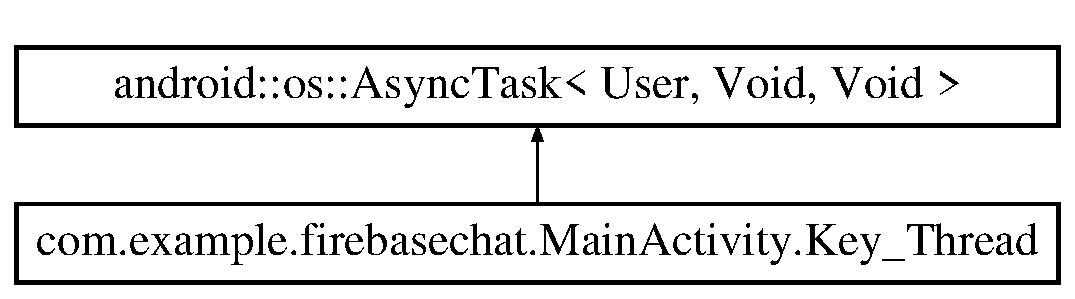
\includegraphics[height=2.000000cm]{classcom_1_1example_1_1firebasechat_1_1_main_activity_1_1_key___thread}
\end{center}
\end{figure}
\subsection*{Защищенные члены}
\begin{DoxyCompactItemize}
\item 
void \mbox{\hyperlink{classcom_1_1example_1_1firebasechat_1_1_main_activity_1_1_key___thread_ab4f5d0fba51cf4688bbb5bcdec87fe57}{on\+Pre\+Execute}} ()
\item 
Void \mbox{\hyperlink{classcom_1_1example_1_1firebasechat_1_1_main_activity_1_1_key___thread_a6e944d0c77208e4ec4f8d18207d78412}{do\+In\+Background}} (\mbox{\hyperlink{classcom_1_1example_1_1firebasechat_1_1_user}{User}} ... \mbox{\hyperlink{classcom_1_1example_1_1firebasechat_1_1_main_activity_a139972aaf697b18799afeede7a832bc0}{current\+\_\+user}})
\item 
void \mbox{\hyperlink{classcom_1_1example_1_1firebasechat_1_1_main_activity_1_1_key___thread_a8b45edd36455a43fe7266f8c49adaf75}{on\+Post\+Execute}} (Void result)
\end{DoxyCompactItemize}


\subsection{Подробное описание}
Поток для обработки генерации ключей 

См. определение в файле Main\+Activity.\+java строка 272



\subsection{Методы}
\mbox{\Hypertarget{classcom_1_1example_1_1firebasechat_1_1_main_activity_1_1_key___thread_a6e944d0c77208e4ec4f8d18207d78412}\label{classcom_1_1example_1_1firebasechat_1_1_main_activity_1_1_key___thread_a6e944d0c77208e4ec4f8d18207d78412}} 
\index{com\+::example\+::firebasechat\+::\+Main\+Activity\+::\+Key\+\_\+\+Thread@{com\+::example\+::firebasechat\+::\+Main\+Activity\+::\+Key\+\_\+\+Thread}!do\+In\+Background@{do\+In\+Background}}
\index{do\+In\+Background@{do\+In\+Background}!com\+::example\+::firebasechat\+::\+Main\+Activity\+::\+Key\+\_\+\+Thread@{com\+::example\+::firebasechat\+::\+Main\+Activity\+::\+Key\+\_\+\+Thread}}
\subsubsection{\texorpdfstring{do\+In\+Background()}{doInBackground()}}
{\footnotesize\ttfamily Void com.\+example.\+firebasechat.\+Main\+Activity.\+Key\+\_\+\+Thread.\+do\+In\+Background (\begin{DoxyParamCaption}\item[{\mbox{\hyperlink{classcom_1_1example_1_1firebasechat_1_1_user}{User}} ...}]{current\+\_\+user }\end{DoxyParamCaption})\hspace{0.3cm}{\ttfamily [protected]}}



См. определение в файле Main\+Activity.\+java строка 284

\mbox{\Hypertarget{classcom_1_1example_1_1firebasechat_1_1_main_activity_1_1_key___thread_a8b45edd36455a43fe7266f8c49adaf75}\label{classcom_1_1example_1_1firebasechat_1_1_main_activity_1_1_key___thread_a8b45edd36455a43fe7266f8c49adaf75}} 
\index{com\+::example\+::firebasechat\+::\+Main\+Activity\+::\+Key\+\_\+\+Thread@{com\+::example\+::firebasechat\+::\+Main\+Activity\+::\+Key\+\_\+\+Thread}!on\+Post\+Execute@{on\+Post\+Execute}}
\index{on\+Post\+Execute@{on\+Post\+Execute}!com\+::example\+::firebasechat\+::\+Main\+Activity\+::\+Key\+\_\+\+Thread@{com\+::example\+::firebasechat\+::\+Main\+Activity\+::\+Key\+\_\+\+Thread}}
\subsubsection{\texorpdfstring{on\+Post\+Execute()}{onPostExecute()}}
{\footnotesize\ttfamily void com.\+example.\+firebasechat.\+Main\+Activity.\+Key\+\_\+\+Thread.\+on\+Post\+Execute (\begin{DoxyParamCaption}\item[{Void}]{result }\end{DoxyParamCaption})\hspace{0.3cm}{\ttfamily [protected]}}



См. определение в файле Main\+Activity.\+java строка 303

\mbox{\Hypertarget{classcom_1_1example_1_1firebasechat_1_1_main_activity_1_1_key___thread_ab4f5d0fba51cf4688bbb5bcdec87fe57}\label{classcom_1_1example_1_1firebasechat_1_1_main_activity_1_1_key___thread_ab4f5d0fba51cf4688bbb5bcdec87fe57}} 
\index{com\+::example\+::firebasechat\+::\+Main\+Activity\+::\+Key\+\_\+\+Thread@{com\+::example\+::firebasechat\+::\+Main\+Activity\+::\+Key\+\_\+\+Thread}!on\+Pre\+Execute@{on\+Pre\+Execute}}
\index{on\+Pre\+Execute@{on\+Pre\+Execute}!com\+::example\+::firebasechat\+::\+Main\+Activity\+::\+Key\+\_\+\+Thread@{com\+::example\+::firebasechat\+::\+Main\+Activity\+::\+Key\+\_\+\+Thread}}
\subsubsection{\texorpdfstring{on\+Pre\+Execute()}{onPreExecute()}}
{\footnotesize\ttfamily void com.\+example.\+firebasechat.\+Main\+Activity.\+Key\+\_\+\+Thread.\+on\+Pre\+Execute (\begin{DoxyParamCaption}{ }\end{DoxyParamCaption})\hspace{0.3cm}{\ttfamily [protected]}}



См. определение в файле Main\+Activity.\+java строка 275



Объявления и описания членов класса находятся в файле\+:\begin{DoxyCompactItemize}
\item 
C\+:/\+Games/\+Back\+Up/\+Fire\+Basechat/app/src/main/java/com/example/firebasechat/\mbox{\hyperlink{_main_activity_8java}{Main\+Activity.\+java}}\end{DoxyCompactItemize}

\hypertarget{classcom_1_1example_1_1firebasechat_1_1_main_activity}{}\section{Класс com.\+example.\+firebasechat.\+Main\+Activity}
\label{classcom_1_1example_1_1firebasechat_1_1_main_activity}\index{com.\+example.\+firebasechat.\+Main\+Activity@{com.\+example.\+firebasechat.\+Main\+Activity}}


Activity регистрации и авторизации пользователей  


Граф наследования\+:com.\+example.\+firebasechat.\+Main\+Activity\+:\begin{figure}[H]
\begin{center}
\leavevmode
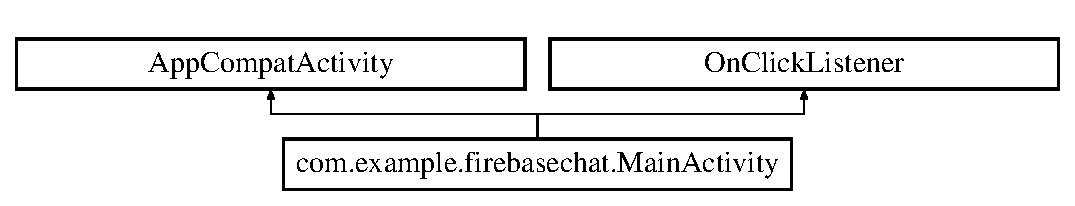
\includegraphics[height=2.000000cm]{classcom_1_1example_1_1firebasechat_1_1_main_activity}
\end{center}
\end{figure}
\subsection*{Классы}
\begin{DoxyCompactItemize}
\item 
class \mbox{\hyperlink{classcom_1_1example_1_1firebasechat_1_1_main_activity_1_1_key___thread}{Key\+\_\+\+Thread}}
\begin{DoxyCompactList}\small\item\em Поток для обработки генерации ключей \end{DoxyCompactList}\end{DoxyCompactItemize}
\subsection*{Открытые члены}
\begin{DoxyCompactItemize}
\item 
void \mbox{\hyperlink{classcom_1_1example_1_1firebasechat_1_1_main_activity_a859bd2e4eca1bcc5b64414f3fae8dfd5}{on\+Click}} (View view)
\item 
void \mbox{\hyperlink{classcom_1_1example_1_1firebasechat_1_1_main_activity_ab05b9f3c667fd2a59b127fdf24f7af8f}{signin}} (String email, final String password\+\_\+)
\begin{DoxyCompactList}\small\item\em Функция, реализующая авторизацию пользователя по паролю и почте \end{DoxyCompactList}\item 
void \mbox{\hyperlink{classcom_1_1example_1_1firebasechat_1_1_main_activity_a95140ec9da54a87bc49b6ba1023cb8bd}{registration}} (String email, String password)
\begin{DoxyCompactList}\small\item\em Функция, реализующая регистрацию пользователя по паролю и почте \end{DoxyCompactList}\item 
void \mbox{\hyperlink{classcom_1_1example_1_1firebasechat_1_1_main_activity_a61ce1168261dbdab070cb0497ad845eb}{keys\+\_\+generation}} ()
\begin{DoxyCompactList}\small\item\em Переотправка ключей для пользователей, у которых нет их на данном устройстве \end{DoxyCompactList}\item 
void \mbox{\hyperlink{classcom_1_1example_1_1firebasechat_1_1_main_activity_abca69f1465f860b8f9eedaa3b360201d}{admin\+\_\+auth}} (String password)
\begin{DoxyCompactList}\small\item\em Авторизация для Администратора \end{DoxyCompactList}\item 
void \mbox{\hyperlink{classcom_1_1example_1_1firebasechat_1_1_main_activity_a4cc4577677e01c9c0898ab0aaa07d670}{user\+\_\+auth}} ()
\begin{DoxyCompactList}\small\item\em Авторизация для пользователей \end{DoxyCompactList}\end{DoxyCompactItemize}
\subsection*{Открытые атрибуты}
\begin{DoxyCompactItemize}
\item 
Database\+Reference \mbox{\hyperlink{classcom_1_1example_1_1firebasechat_1_1_main_activity_a058a21d2029c7bfbb3365c50b621e043}{pkeys}} = Firebase\+Database.\+get\+Instance().get\+Reference(\char`\"{}Public\+\_\+\+Key\char`\"{})
\begin{DoxyCompactList}\small\item\em Базад данных публичных ключей \end{DoxyCompactList}\end{DoxyCompactItemize}
\subsection*{Статические открытые данные}
\begin{DoxyCompactItemize}
\item 
static \mbox{\hyperlink{classcom_1_1example_1_1firebasechat_1_1_user}{User}} \mbox{\hyperlink{classcom_1_1example_1_1firebasechat_1_1_main_activity_a139972aaf697b18799afeede7a832bc0}{current\+\_\+user}}
\begin{DoxyCompactList}\small\item\em Пользователь \end{DoxyCompactList}\end{DoxyCompactItemize}
\subsection*{Защищенные члены}
\begin{DoxyCompactItemize}
\item 
void \mbox{\hyperlink{classcom_1_1example_1_1firebasechat_1_1_main_activity_a65ecbc7b4bebeeee38c9e5ae03720412}{on\+Create}} (Bundle saved\+Instance\+State)
\begin{DoxyCompactList}\small\item\em Создание activity \mbox{\hyperlink{classcom_1_1example_1_1firebasechat_1_1_main_activity}{Main\+Activity}}. \end{DoxyCompactList}\end{DoxyCompactItemize}


\subsection{Подробное описание}
Activity регистрации и авторизации пользователей 

Данное Activity предназначено для регистрации или авторизации пользователя, также содержит кнопку перехода на страницу информации об авторах 

См. определение в файле Main\+Activity.\+java строка 47



\subsection{Методы}
\mbox{\Hypertarget{classcom_1_1example_1_1firebasechat_1_1_main_activity_abca69f1465f860b8f9eedaa3b360201d}\label{classcom_1_1example_1_1firebasechat_1_1_main_activity_abca69f1465f860b8f9eedaa3b360201d}} 
\index{com\+::example\+::firebasechat\+::\+Main\+Activity@{com\+::example\+::firebasechat\+::\+Main\+Activity}!admin\+\_\+auth@{admin\+\_\+auth}}
\index{admin\+\_\+auth@{admin\+\_\+auth}!com\+::example\+::firebasechat\+::\+Main\+Activity@{com\+::example\+::firebasechat\+::\+Main\+Activity}}
\subsubsection{\texorpdfstring{admin\+\_\+auth()}{admin\_auth()}}
{\footnotesize\ttfamily void com.\+example.\+firebasechat.\+Main\+Activity.\+admin\+\_\+auth (\begin{DoxyParamCaption}\item[{String}]{password }\end{DoxyParamCaption})}



Авторизация для Администратора 


\begin{DoxyParams}{Аргументы}
{\em password} & \\
\hline
\end{DoxyParams}


См. определение в файле Main\+Activity.\+java строка 196

\mbox{\Hypertarget{classcom_1_1example_1_1firebasechat_1_1_main_activity_a61ce1168261dbdab070cb0497ad845eb}\label{classcom_1_1example_1_1firebasechat_1_1_main_activity_a61ce1168261dbdab070cb0497ad845eb}} 
\index{com\+::example\+::firebasechat\+::\+Main\+Activity@{com\+::example\+::firebasechat\+::\+Main\+Activity}!keys\+\_\+generation@{keys\+\_\+generation}}
\index{keys\+\_\+generation@{keys\+\_\+generation}!com\+::example\+::firebasechat\+::\+Main\+Activity@{com\+::example\+::firebasechat\+::\+Main\+Activity}}
\subsubsection{\texorpdfstring{keys\+\_\+generation()}{keys\_generation()}}
{\footnotesize\ttfamily void com.\+example.\+firebasechat.\+Main\+Activity.\+keys\+\_\+generation (\begin{DoxyParamCaption}{ }\end{DoxyParamCaption})}



Переотправка ключей для пользователей, у которых нет их на данном устройстве 



См. определение в файле Main\+Activity.\+java строка 179

\mbox{\Hypertarget{classcom_1_1example_1_1firebasechat_1_1_main_activity_a859bd2e4eca1bcc5b64414f3fae8dfd5}\label{classcom_1_1example_1_1firebasechat_1_1_main_activity_a859bd2e4eca1bcc5b64414f3fae8dfd5}} 
\index{com\+::example\+::firebasechat\+::\+Main\+Activity@{com\+::example\+::firebasechat\+::\+Main\+Activity}!on\+Click@{on\+Click}}
\index{on\+Click@{on\+Click}!com\+::example\+::firebasechat\+::\+Main\+Activity@{com\+::example\+::firebasechat\+::\+Main\+Activity}}
\subsubsection{\texorpdfstring{on\+Click()}{onClick()}}
{\footnotesize\ttfamily void com.\+example.\+firebasechat.\+Main\+Activity.\+on\+Click (\begin{DoxyParamCaption}\item[{View}]{view }\end{DoxyParamCaption})}



См. определение в файле Main\+Activity.\+java строка 104

\mbox{\Hypertarget{classcom_1_1example_1_1firebasechat_1_1_main_activity_a65ecbc7b4bebeeee38c9e5ae03720412}\label{classcom_1_1example_1_1firebasechat_1_1_main_activity_a65ecbc7b4bebeeee38c9e5ae03720412}} 
\index{com\+::example\+::firebasechat\+::\+Main\+Activity@{com\+::example\+::firebasechat\+::\+Main\+Activity}!on\+Create@{on\+Create}}
\index{on\+Create@{on\+Create}!com\+::example\+::firebasechat\+::\+Main\+Activity@{com\+::example\+::firebasechat\+::\+Main\+Activity}}
\subsubsection{\texorpdfstring{on\+Create()}{onCreate()}}
{\footnotesize\ttfamily void com.\+example.\+firebasechat.\+Main\+Activity.\+on\+Create (\begin{DoxyParamCaption}\item[{Bundle}]{saved\+Instance\+State }\end{DoxyParamCaption})\hspace{0.3cm}{\ttfamily [protected]}}



Создание activity \mbox{\hyperlink{classcom_1_1example_1_1firebasechat_1_1_main_activity}{Main\+Activity}}. 


\begin{DoxyParams}{Аргументы}
{\em saved\+Instance\+State} & \\
\hline
\end{DoxyParams}


См. определение в файле Main\+Activity.\+java строка 78

\mbox{\Hypertarget{classcom_1_1example_1_1firebasechat_1_1_main_activity_a95140ec9da54a87bc49b6ba1023cb8bd}\label{classcom_1_1example_1_1firebasechat_1_1_main_activity_a95140ec9da54a87bc49b6ba1023cb8bd}} 
\index{com\+::example\+::firebasechat\+::\+Main\+Activity@{com\+::example\+::firebasechat\+::\+Main\+Activity}!registration@{registration}}
\index{registration@{registration}!com\+::example\+::firebasechat\+::\+Main\+Activity@{com\+::example\+::firebasechat\+::\+Main\+Activity}}
\subsubsection{\texorpdfstring{registration()}{registration()}}
{\footnotesize\ttfamily void com.\+example.\+firebasechat.\+Main\+Activity.\+registration (\begin{DoxyParamCaption}\item[{String}]{email,  }\item[{String}]{password }\end{DoxyParamCaption})}



Функция, реализующая регистрацию пользователя по паролю и почте 

При успешной регистрации для пользователя генерируются ключи, которые после генерации отправляются на сервер 
\begin{DoxyParams}{Аргументы}
{\em email} & Данный, который пользователь ввел в поле почты \\
\hline
{\em password} & Данный, который пользователь ввел в поле пароля \\
\hline
\end{DoxyParams}


См. определение в файле Main\+Activity.\+java строка 162

\mbox{\Hypertarget{classcom_1_1example_1_1firebasechat_1_1_main_activity_ab05b9f3c667fd2a59b127fdf24f7af8f}\label{classcom_1_1example_1_1firebasechat_1_1_main_activity_ab05b9f3c667fd2a59b127fdf24f7af8f}} 
\index{com\+::example\+::firebasechat\+::\+Main\+Activity@{com\+::example\+::firebasechat\+::\+Main\+Activity}!signin@{signin}}
\index{signin@{signin}!com\+::example\+::firebasechat\+::\+Main\+Activity@{com\+::example\+::firebasechat\+::\+Main\+Activity}}
\subsubsection{\texorpdfstring{signin()}{signin()}}
{\footnotesize\ttfamily void com.\+example.\+firebasechat.\+Main\+Activity.\+signin (\begin{DoxyParamCaption}\item[{String}]{email,  }\item[{final String}]{password\+\_\+ }\end{DoxyParamCaption})}



Функция, реализующая авторизацию пользователя по паролю и почте 


\begin{DoxyParams}{Аргументы}
{\em email} & Данный, который пользователь ввел в поле почты \\
\hline
{\em password} & Данный, который пользователь ввел в поле пароля \\
\hline
\end{DoxyParams}


См. определение в файле Main\+Activity.\+java строка 137

\mbox{\Hypertarget{classcom_1_1example_1_1firebasechat_1_1_main_activity_a4cc4577677e01c9c0898ab0aaa07d670}\label{classcom_1_1example_1_1firebasechat_1_1_main_activity_a4cc4577677e01c9c0898ab0aaa07d670}} 
\index{com\+::example\+::firebasechat\+::\+Main\+Activity@{com\+::example\+::firebasechat\+::\+Main\+Activity}!user\+\_\+auth@{user\+\_\+auth}}
\index{user\+\_\+auth@{user\+\_\+auth}!com\+::example\+::firebasechat\+::\+Main\+Activity@{com\+::example\+::firebasechat\+::\+Main\+Activity}}
\subsubsection{\texorpdfstring{user\+\_\+auth()}{user\_auth()}}
{\footnotesize\ttfamily void com.\+example.\+firebasechat.\+Main\+Activity.\+user\+\_\+auth (\begin{DoxyParamCaption}{ }\end{DoxyParamCaption})}



Авторизация для пользователей 



См. определение в файле Main\+Activity.\+java строка 242



\subsection{Данные класса}
\mbox{\Hypertarget{classcom_1_1example_1_1firebasechat_1_1_main_activity_a139972aaf697b18799afeede7a832bc0}\label{classcom_1_1example_1_1firebasechat_1_1_main_activity_a139972aaf697b18799afeede7a832bc0}} 
\index{com\+::example\+::firebasechat\+::\+Main\+Activity@{com\+::example\+::firebasechat\+::\+Main\+Activity}!current\+\_\+user@{current\+\_\+user}}
\index{current\+\_\+user@{current\+\_\+user}!com\+::example\+::firebasechat\+::\+Main\+Activity@{com\+::example\+::firebasechat\+::\+Main\+Activity}}
\subsubsection{\texorpdfstring{current\+\_\+user}{current\_user}}
{\footnotesize\ttfamily \mbox{\hyperlink{classcom_1_1example_1_1firebasechat_1_1_user}{User}} com.\+example.\+firebasechat.\+Main\+Activity.\+current\+\_\+user\hspace{0.3cm}{\ttfamily [static]}}



Пользователь 



См. определение в файле Main\+Activity.\+java строка 67

\mbox{\Hypertarget{classcom_1_1example_1_1firebasechat_1_1_main_activity_a058a21d2029c7bfbb3365c50b621e043}\label{classcom_1_1example_1_1firebasechat_1_1_main_activity_a058a21d2029c7bfbb3365c50b621e043}} 
\index{com\+::example\+::firebasechat\+::\+Main\+Activity@{com\+::example\+::firebasechat\+::\+Main\+Activity}!pkeys@{pkeys}}
\index{pkeys@{pkeys}!com\+::example\+::firebasechat\+::\+Main\+Activity@{com\+::example\+::firebasechat\+::\+Main\+Activity}}
\subsubsection{\texorpdfstring{pkeys}{pkeys}}
{\footnotesize\ttfamily Database\+Reference com.\+example.\+firebasechat.\+Main\+Activity.\+pkeys = Firebase\+Database.\+get\+Instance().get\+Reference(\char`\"{}Public\+\_\+\+Key\char`\"{})}



Базад данных публичных ключей 



См. определение в файле Main\+Activity.\+java строка 69



Объявления и описания членов класса находятся в файле\+:\begin{DoxyCompactItemize}
\item 
C\+:/\+Games/\+Back\+Up/\+Fire\+Basechat/app/src/main/java/com/example/firebasechat/\mbox{\hyperlink{_main_activity_8java}{Main\+Activity.\+java}}\end{DoxyCompactItemize}

\hypertarget{classcom_1_1example_1_1firebasechat_1_1_message}{}\section{Класс com.\+example.\+firebasechat.\+Message}
\label{classcom_1_1example_1_1firebasechat_1_1_message}\index{com.\+example.\+firebasechat.\+Message@{com.\+example.\+firebasechat.\+Message}}


Класс сообщений пользователей  


\subsection*{Открытые члены}
\begin{DoxyCompactItemize}
\item 
\mbox{\hyperlink{classcom_1_1example_1_1firebasechat_1_1_message_a16d2a1e81245c95a65287af20c897bcf}{Message}} (String \mbox{\hyperlink{classcom_1_1example_1_1firebasechat_1_1_message_acb2c8f619df31749afdc79e92b1481e8}{text\+Message}}, String \mbox{\hyperlink{classcom_1_1example_1_1firebasechat_1_1_message_a8d952ef9a02a74e7c419f335020fea23}{author}})
\begin{DoxyCompactList}\small\item\em Конструктор класса \mbox{\hyperlink{classcom_1_1example_1_1firebasechat_1_1_message}{Message}}. \end{DoxyCompactList}\item 
\mbox{\hyperlink{classcom_1_1example_1_1firebasechat_1_1_message_a6693707a10383562d63555ee5014a9aa}{Message}} ()
\item 
String \mbox{\hyperlink{classcom_1_1example_1_1firebasechat_1_1_message_aefada8da06d095f5c982ec8b556d6554}{get\+Text\+Message}} ()
\item 
void \mbox{\hyperlink{classcom_1_1example_1_1firebasechat_1_1_message_abb5288c3d6bd3e961f9ee1f7680abb65}{set\+Text\+Message}} (String \mbox{\hyperlink{classcom_1_1example_1_1firebasechat_1_1_message_acb2c8f619df31749afdc79e92b1481e8}{text\+Message}})
\begin{DoxyCompactList}\small\item\em Setter для текста сообщения \end{DoxyCompactList}\item 
String \mbox{\hyperlink{classcom_1_1example_1_1firebasechat_1_1_message_a13ca75f96f4b6c16a83190b1ff8f819f}{get\+Author}} ()
\begin{DoxyCompactList}\small\item\em Getter для автора \end{DoxyCompactList}\item 
void \mbox{\hyperlink{classcom_1_1example_1_1firebasechat_1_1_message_a8fd45837a4a4bd7682909d5c8d4d11b6}{set\+Author}} (String \mbox{\hyperlink{classcom_1_1example_1_1firebasechat_1_1_message_a8d952ef9a02a74e7c419f335020fea23}{author}})
\begin{DoxyCompactList}\small\item\em Setter для авора \end{DoxyCompactList}\item 
String \mbox{\hyperlink{classcom_1_1example_1_1firebasechat_1_1_message_a3616de6e6cf9ddcfee8b09ac520133e4}{get\+Time\+Message\+String}} ()
\begin{DoxyCompactList}\small\item\em Getter для времени сообщения в формате String. \end{DoxyCompactList}\item 
long \mbox{\hyperlink{classcom_1_1example_1_1firebasechat_1_1_message_a3c210d1ca7c8582e702aff4c1e6fdd47}{get\+Time\+Message}} ()
\begin{DoxyCompactList}\small\item\em Getter для времени сообщения \end{DoxyCompactList}\item 
void \mbox{\hyperlink{classcom_1_1example_1_1firebasechat_1_1_message_a49fdc6fad71c37aa636d43400c8c63bc}{set\+Time\+Message}} (long \mbox{\hyperlink{classcom_1_1example_1_1firebasechat_1_1_message_a09635d0a02cd29c65625d1d1c2a616a3}{time\+Message}})
\begin{DoxyCompactList}\small\item\em Setter для времени сообщения \end{DoxyCompactList}\end{DoxyCompactItemize}
\subsection*{Открытые атрибуты}
\begin{DoxyCompactItemize}
\item 
String \mbox{\hyperlink{classcom_1_1example_1_1firebasechat_1_1_message_acb2c8f619df31749afdc79e92b1481e8}{text\+Message}}
\begin{DoxyCompactList}\small\item\em Текст сообщения \end{DoxyCompactList}\item 
String \mbox{\hyperlink{classcom_1_1example_1_1firebasechat_1_1_message_a8d952ef9a02a74e7c419f335020fea23}{author}}
\begin{DoxyCompactList}\small\item\em Автор сообщения \end{DoxyCompactList}\item 
long \mbox{\hyperlink{classcom_1_1example_1_1firebasechat_1_1_message_a09635d0a02cd29c65625d1d1c2a616a3}{time\+Message}}
\begin{DoxyCompactList}\small\item\em Время отправки сообщения \end{DoxyCompactList}\end{DoxyCompactItemize}


\subsection{Подробное описание}
Класс сообщений пользователей 

См. определение в файле Message.\+java строка 7



\subsection{Конструктор(ы)}
\mbox{\Hypertarget{classcom_1_1example_1_1firebasechat_1_1_message_a16d2a1e81245c95a65287af20c897bcf}\label{classcom_1_1example_1_1firebasechat_1_1_message_a16d2a1e81245c95a65287af20c897bcf}} 
\index{com\+::example\+::firebasechat\+::\+Message@{com\+::example\+::firebasechat\+::\+Message}!Message@{Message}}
\index{Message@{Message}!com\+::example\+::firebasechat\+::\+Message@{com\+::example\+::firebasechat\+::\+Message}}
\subsubsection{\texorpdfstring{Message()}{Message()}\hspace{0.1cm}{\footnotesize\ttfamily [1/2]}}
{\footnotesize\ttfamily com.\+example.\+firebasechat.\+Message.\+Message (\begin{DoxyParamCaption}\item[{String}]{text\+Message,  }\item[{String}]{author }\end{DoxyParamCaption})}



Конструктор класса \mbox{\hyperlink{classcom_1_1example_1_1firebasechat_1_1_message}{Message}}. 


\begin{DoxyParams}{Аргументы}
{\em text\+Message} & Текст сообщения \\
\hline
{\em author} & Автор сообщения \\
\hline
\end{DoxyParams}


См. определение в файле Message.\+java строка 18

\mbox{\Hypertarget{classcom_1_1example_1_1firebasechat_1_1_message_a6693707a10383562d63555ee5014a9aa}\label{classcom_1_1example_1_1firebasechat_1_1_message_a6693707a10383562d63555ee5014a9aa}} 
\index{com\+::example\+::firebasechat\+::\+Message@{com\+::example\+::firebasechat\+::\+Message}!Message@{Message}}
\index{Message@{Message}!com\+::example\+::firebasechat\+::\+Message@{com\+::example\+::firebasechat\+::\+Message}}
\subsubsection{\texorpdfstring{Message()}{Message()}\hspace{0.1cm}{\footnotesize\ttfamily [2/2]}}
{\footnotesize\ttfamily com.\+example.\+firebasechat.\+Message.\+Message (\begin{DoxyParamCaption}{ }\end{DoxyParamCaption})}



См. определение в файле Message.\+java строка 24



\subsection{Методы}
\mbox{\Hypertarget{classcom_1_1example_1_1firebasechat_1_1_message_a13ca75f96f4b6c16a83190b1ff8f819f}\label{classcom_1_1example_1_1firebasechat_1_1_message_a13ca75f96f4b6c16a83190b1ff8f819f}} 
\index{com\+::example\+::firebasechat\+::\+Message@{com\+::example\+::firebasechat\+::\+Message}!get\+Author@{get\+Author}}
\index{get\+Author@{get\+Author}!com\+::example\+::firebasechat\+::\+Message@{com\+::example\+::firebasechat\+::\+Message}}
\subsubsection{\texorpdfstring{get\+Author()}{getAuthor()}}
{\footnotesize\ttfamily String com.\+example.\+firebasechat.\+Message.\+get\+Author (\begin{DoxyParamCaption}{ }\end{DoxyParamCaption})}



Getter для автора 

\begin{DoxyReturn}{Возвращает}
Автор 
\end{DoxyReturn}


См. определение в файле Message.\+java строка 47

\mbox{\Hypertarget{classcom_1_1example_1_1firebasechat_1_1_message_aefada8da06d095f5c982ec8b556d6554}\label{classcom_1_1example_1_1firebasechat_1_1_message_aefada8da06d095f5c982ec8b556d6554}} 
\index{com\+::example\+::firebasechat\+::\+Message@{com\+::example\+::firebasechat\+::\+Message}!get\+Text\+Message@{get\+Text\+Message}}
\index{get\+Text\+Message@{get\+Text\+Message}!com\+::example\+::firebasechat\+::\+Message@{com\+::example\+::firebasechat\+::\+Message}}
\subsubsection{\texorpdfstring{get\+Text\+Message()}{getTextMessage()}}
{\footnotesize\ttfamily String com.\+example.\+firebasechat.\+Message.\+get\+Text\+Message (\begin{DoxyParamCaption}{ }\end{DoxyParamCaption})}

Getter для текста сообщения \begin{DoxyReturn}{Возвращает}
Текст сообщения 
\end{DoxyReturn}


См. определение в файле Message.\+java строка 31

\mbox{\Hypertarget{classcom_1_1example_1_1firebasechat_1_1_message_a3c210d1ca7c8582e702aff4c1e6fdd47}\label{classcom_1_1example_1_1firebasechat_1_1_message_a3c210d1ca7c8582e702aff4c1e6fdd47}} 
\index{com\+::example\+::firebasechat\+::\+Message@{com\+::example\+::firebasechat\+::\+Message}!get\+Time\+Message@{get\+Time\+Message}}
\index{get\+Time\+Message@{get\+Time\+Message}!com\+::example\+::firebasechat\+::\+Message@{com\+::example\+::firebasechat\+::\+Message}}
\subsubsection{\texorpdfstring{get\+Time\+Message()}{getTimeMessage()}}
{\footnotesize\ttfamily long com.\+example.\+firebasechat.\+Message.\+get\+Time\+Message (\begin{DoxyParamCaption}{ }\end{DoxyParamCaption})}



Getter для времени сообщения 

\begin{DoxyReturn}{Возвращает}
Время сообщения 
\end{DoxyReturn}


См. определение в файле Message.\+java строка 71

\mbox{\Hypertarget{classcom_1_1example_1_1firebasechat_1_1_message_a3616de6e6cf9ddcfee8b09ac520133e4}\label{classcom_1_1example_1_1firebasechat_1_1_message_a3616de6e6cf9ddcfee8b09ac520133e4}} 
\index{com\+::example\+::firebasechat\+::\+Message@{com\+::example\+::firebasechat\+::\+Message}!get\+Time\+Message\+String@{get\+Time\+Message\+String}}
\index{get\+Time\+Message\+String@{get\+Time\+Message\+String}!com\+::example\+::firebasechat\+::\+Message@{com\+::example\+::firebasechat\+::\+Message}}
\subsubsection{\texorpdfstring{get\+Time\+Message\+String()}{getTimeMessageString()}}
{\footnotesize\ttfamily String com.\+example.\+firebasechat.\+Message.\+get\+Time\+Message\+String (\begin{DoxyParamCaption}{ }\end{DoxyParamCaption})}



Getter для времени сообщения в формате String. 

\begin{DoxyReturn}{Возвращает}
Время сообщения 
\end{DoxyReturn}


См. определение в файле Message.\+java строка 63

\mbox{\Hypertarget{classcom_1_1example_1_1firebasechat_1_1_message_a8fd45837a4a4bd7682909d5c8d4d11b6}\label{classcom_1_1example_1_1firebasechat_1_1_message_a8fd45837a4a4bd7682909d5c8d4d11b6}} 
\index{com\+::example\+::firebasechat\+::\+Message@{com\+::example\+::firebasechat\+::\+Message}!set\+Author@{set\+Author}}
\index{set\+Author@{set\+Author}!com\+::example\+::firebasechat\+::\+Message@{com\+::example\+::firebasechat\+::\+Message}}
\subsubsection{\texorpdfstring{set\+Author()}{setAuthor()}}
{\footnotesize\ttfamily void com.\+example.\+firebasechat.\+Message.\+set\+Author (\begin{DoxyParamCaption}\item[{String}]{author }\end{DoxyParamCaption})}



Setter для авора 


\begin{DoxyParams}{Аргументы}
{\em author} & Автор \\
\hline
\end{DoxyParams}


См. определение в файле Message.\+java строка 55

\mbox{\Hypertarget{classcom_1_1example_1_1firebasechat_1_1_message_abb5288c3d6bd3e961f9ee1f7680abb65}\label{classcom_1_1example_1_1firebasechat_1_1_message_abb5288c3d6bd3e961f9ee1f7680abb65}} 
\index{com\+::example\+::firebasechat\+::\+Message@{com\+::example\+::firebasechat\+::\+Message}!set\+Text\+Message@{set\+Text\+Message}}
\index{set\+Text\+Message@{set\+Text\+Message}!com\+::example\+::firebasechat\+::\+Message@{com\+::example\+::firebasechat\+::\+Message}}
\subsubsection{\texorpdfstring{set\+Text\+Message()}{setTextMessage()}}
{\footnotesize\ttfamily void com.\+example.\+firebasechat.\+Message.\+set\+Text\+Message (\begin{DoxyParamCaption}\item[{String}]{text\+Message }\end{DoxyParamCaption})}



Setter для текста сообщения 


\begin{DoxyParams}{Аргументы}
{\em text\+Message} & Текст сообщения \\
\hline
\end{DoxyParams}


См. определение в файле Message.\+java строка 39

\mbox{\Hypertarget{classcom_1_1example_1_1firebasechat_1_1_message_a49fdc6fad71c37aa636d43400c8c63bc}\label{classcom_1_1example_1_1firebasechat_1_1_message_a49fdc6fad71c37aa636d43400c8c63bc}} 
\index{com\+::example\+::firebasechat\+::\+Message@{com\+::example\+::firebasechat\+::\+Message}!set\+Time\+Message@{set\+Time\+Message}}
\index{set\+Time\+Message@{set\+Time\+Message}!com\+::example\+::firebasechat\+::\+Message@{com\+::example\+::firebasechat\+::\+Message}}
\subsubsection{\texorpdfstring{set\+Time\+Message()}{setTimeMessage()}}
{\footnotesize\ttfamily void com.\+example.\+firebasechat.\+Message.\+set\+Time\+Message (\begin{DoxyParamCaption}\item[{long}]{time\+Message }\end{DoxyParamCaption})}



Setter для времени сообщения 


\begin{DoxyParams}{Аргументы}
{\em time\+Message} & время сообщения \\
\hline
\end{DoxyParams}


См. определение в файле Message.\+java строка 77



\subsection{Данные класса}
\mbox{\Hypertarget{classcom_1_1example_1_1firebasechat_1_1_message_a8d952ef9a02a74e7c419f335020fea23}\label{classcom_1_1example_1_1firebasechat_1_1_message_a8d952ef9a02a74e7c419f335020fea23}} 
\index{com\+::example\+::firebasechat\+::\+Message@{com\+::example\+::firebasechat\+::\+Message}!author@{author}}
\index{author@{author}!com\+::example\+::firebasechat\+::\+Message@{com\+::example\+::firebasechat\+::\+Message}}
\subsubsection{\texorpdfstring{author}{author}}
{\footnotesize\ttfamily String com.\+example.\+firebasechat.\+Message.\+author}



Автор сообщения 



См. определение в файле Message.\+java строка 10

\mbox{\Hypertarget{classcom_1_1example_1_1firebasechat_1_1_message_acb2c8f619df31749afdc79e92b1481e8}\label{classcom_1_1example_1_1firebasechat_1_1_message_acb2c8f619df31749afdc79e92b1481e8}} 
\index{com\+::example\+::firebasechat\+::\+Message@{com\+::example\+::firebasechat\+::\+Message}!text\+Message@{text\+Message}}
\index{text\+Message@{text\+Message}!com\+::example\+::firebasechat\+::\+Message@{com\+::example\+::firebasechat\+::\+Message}}
\subsubsection{\texorpdfstring{text\+Message}{textMessage}}
{\footnotesize\ttfamily String com.\+example.\+firebasechat.\+Message.\+text\+Message}



Текст сообщения 



См. определение в файле Message.\+java строка 9

\mbox{\Hypertarget{classcom_1_1example_1_1firebasechat_1_1_message_a09635d0a02cd29c65625d1d1c2a616a3}\label{classcom_1_1example_1_1firebasechat_1_1_message_a09635d0a02cd29c65625d1d1c2a616a3}} 
\index{com\+::example\+::firebasechat\+::\+Message@{com\+::example\+::firebasechat\+::\+Message}!time\+Message@{time\+Message}}
\index{time\+Message@{time\+Message}!com\+::example\+::firebasechat\+::\+Message@{com\+::example\+::firebasechat\+::\+Message}}
\subsubsection{\texorpdfstring{time\+Message}{timeMessage}}
{\footnotesize\ttfamily long com.\+example.\+firebasechat.\+Message.\+time\+Message}



Время отправки сообщения 



См. определение в файле Message.\+java строка 11



Объявления и описания членов класса находятся в файле\+:\begin{DoxyCompactItemize}
\item 
C\+:/\+Games/\+Back\+Up/\+Fire\+Basechat/app/src/main/java/com/example/firebasechat/\mbox{\hyperlink{_message_8java}{Message.\+java}}\end{DoxyCompactItemize}

\hypertarget{classcom_1_1example_1_1firebasechat_1_1_splash_activity}{}\section{Класс com.\+example.\+firebasechat.\+Splash\+Activity}
\label{classcom_1_1example_1_1firebasechat_1_1_splash_activity}\index{com.\+example.\+firebasechat.\+Splash\+Activity@{com.\+example.\+firebasechat.\+Splash\+Activity}}


Заставка приложения  


Граф наследования\+:com.\+example.\+firebasechat.\+Splash\+Activity\+:\begin{figure}[H]
\begin{center}
\leavevmode
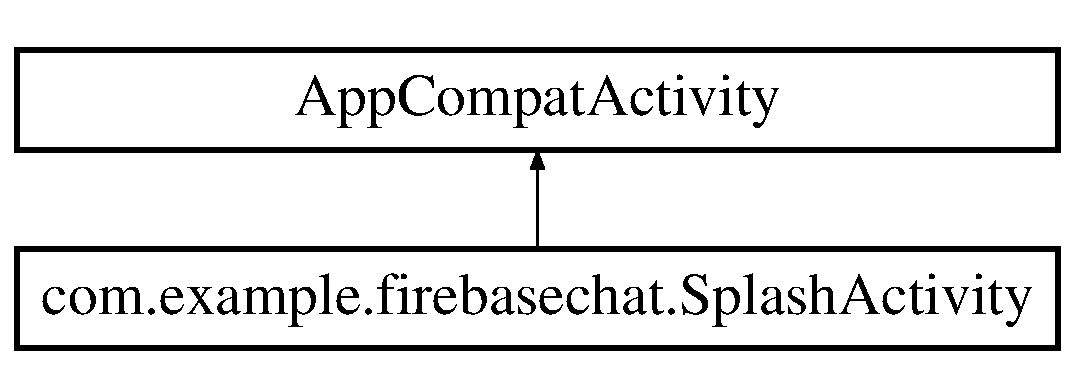
\includegraphics[height=2.000000cm]{classcom_1_1example_1_1firebasechat_1_1_splash_activity}
\end{center}
\end{figure}
\subsection*{Защищенные члены}
\begin{DoxyCompactItemize}
\item 
void \mbox{\hyperlink{classcom_1_1example_1_1firebasechat_1_1_splash_activity_aa1db23df2ab2a3a5506f29e01d054f84}{on\+Create}} (Bundle saved\+Instance\+State)
\begin{DoxyCompactList}\small\item\em Создание activity \mbox{\hyperlink{classcom_1_1example_1_1firebasechat_1_1_splash_activity}{Splash\+Activity}}. \end{DoxyCompactList}\end{DoxyCompactItemize}


\subsection{Подробное описание}
Заставка приложения 

См. определение в файле Splash\+Activity.\+java строка 10



\subsection{Методы}
\mbox{\Hypertarget{classcom_1_1example_1_1firebasechat_1_1_splash_activity_aa1db23df2ab2a3a5506f29e01d054f84}\label{classcom_1_1example_1_1firebasechat_1_1_splash_activity_aa1db23df2ab2a3a5506f29e01d054f84}} 
\index{com\+::example\+::firebasechat\+::\+Splash\+Activity@{com\+::example\+::firebasechat\+::\+Splash\+Activity}!on\+Create@{on\+Create}}
\index{on\+Create@{on\+Create}!com\+::example\+::firebasechat\+::\+Splash\+Activity@{com\+::example\+::firebasechat\+::\+Splash\+Activity}}
\subsubsection{\texorpdfstring{on\+Create()}{onCreate()}}
{\footnotesize\ttfamily void com.\+example.\+firebasechat.\+Splash\+Activity.\+on\+Create (\begin{DoxyParamCaption}\item[{Bundle}]{saved\+Instance\+State }\end{DoxyParamCaption})\hspace{0.3cm}{\ttfamily [protected]}}



Создание activity \mbox{\hyperlink{classcom_1_1example_1_1firebasechat_1_1_splash_activity}{Splash\+Activity}}. 


\begin{DoxyParams}{Аргументы}
{\em saved\+Instance\+State} & \\
\hline
\end{DoxyParams}


См. определение в файле Splash\+Activity.\+java строка 17



Объявления и описания членов класса находятся в файле\+:\begin{DoxyCompactItemize}
\item 
C\+:/\+Games/\+Back\+Up/\+Fire\+Basechat/app/src/main/java/com/example/firebasechat/\mbox{\hyperlink{_splash_activity_8java}{Splash\+Activity.\+java}}\end{DoxyCompactItemize}

\hypertarget{classcom_1_1example_1_1firebasechat_1_1_user}{}\section{Класс com.\+example.\+firebasechat.\+User}
\label{classcom_1_1example_1_1firebasechat_1_1_user}\index{com.\+example.\+firebasechat.\+User@{com.\+example.\+firebasechat.\+User}}


Класс пользователя  


\subsection*{Открытые члены}
\begin{DoxyCompactItemize}
\item 
\mbox{\hyperlink{classcom_1_1example_1_1firebasechat_1_1_user_adc3b037f7e367a6aa8aaac01360d5340}{User}} ()
\begin{DoxyCompactList}\small\item\em Конструктор класса \mbox{\hyperlink{classcom_1_1example_1_1firebasechat_1_1_user}{User}}. \end{DoxyCompactList}\item 
void \mbox{\hyperlink{classcom_1_1example_1_1firebasechat_1_1_user_aa46d2b146ffd91c6b9cf36ec5e194b1f}{set\+Session\+Pair\+\_\+}} (String\mbox{[}$\,$\mbox{]} \mbox{\hyperlink{classcom_1_1example_1_1firebasechat_1_1_user_a2e442876539909f5f9725196556d5fa7}{session\+Pair\+\_\+}})
\begin{DoxyCompactList}\small\item\em Установка сессионных ключей \end{DoxyCompactList}\item 
String \mbox{\hyperlink{classcom_1_1example_1_1firebasechat_1_1_user_af9252d4d96f56d8a74611553307df0a8}{get\+User\+Pub\+Key\+Enc\+Str}} ()
\begin{DoxyCompactList}\small\item\em Getter для публичного ключа \end{DoxyCompactList}\item 
String \mbox{\hyperlink{classcom_1_1example_1_1firebasechat_1_1_user_a6dc80a46d2e49d8c03299dc5b7b15727}{get\+User\+Private\+Key\+Enc\+Str}} ()
\begin{DoxyCompactList}\small\item\em Getter для приватного ключа \end{DoxyCompactList}\item 
void \mbox{\hyperlink{classcom_1_1example_1_1firebasechat_1_1_user_aecc22b4b773ae3ba00ad0c7ed4db4340}{set\+User\+Pub\+Key\+Enc\+Str}} (String \mbox{\hyperlink{classcom_1_1example_1_1firebasechat_1_1_user_a92f14106f35b17ca627b7a5ca0dd3d02}{user\+Pub\+Key\+Enc\+Str}})
\begin{DoxyCompactList}\small\item\em Setter для публичного ключа \end{DoxyCompactList}\item 
void \mbox{\hyperlink{classcom_1_1example_1_1firebasechat_1_1_user_a4cef7096288a776f77934c2cd8f84a72}{set\+User\+Private\+Key\+Enc\+Str}} (String \mbox{\hyperlink{classcom_1_1example_1_1firebasechat_1_1_user_a210e28a59a8e53a7deb7e18027875173}{user\+Private\+Key\+Enc\+Str}})
\begin{DoxyCompactList}\small\item\em Setter для приватного ключа \end{DoxyCompactList}\item 
void \mbox{\hyperlink{classcom_1_1example_1_1firebasechat_1_1_user_a9b6df56e1fc82db7c8d24e81d2250801}{Encrypt\+Session}} (String\mbox{[}$\,$\mbox{]} result)
\begin{DoxyCompactList}\small\item\em Функкция обрабоки пользователем данных, полученных от администратора Пользователь получает данные администратора, генерирует общий секрет и получаает сессионные ключи \end{DoxyCompactList}\item 
String \mbox{[}$\,$\mbox{]} \mbox{\hyperlink{classcom_1_1example_1_1firebasechat_1_1_user_a67d1a7cbc2c9380c36a61503eb44b30f}{D\+H\+Generate\+Admin}} (String \mbox{\hyperlink{classcom_1_1example_1_1firebasechat_1_1_user_a92f14106f35b17ca627b7a5ca0dd3d02}{user\+Pub\+Key\+Enc\+Str}})
\begin{DoxyCompactList}\small\item\em Функция Администратора, где обрабатывается публичный клч пользователя и создаются необходимые ключи \end{DoxyCompactList}\item 
String \mbox{\hyperlink{classcom_1_1example_1_1firebasechat_1_1_user_a7f85ab138092dde2b7f24fc263aaa8ae}{encrypt}} (String value)
\begin{DoxyCompactList}\small\item\em Функция шифрования сообщения \end{DoxyCompactList}\item 
String \mbox{\hyperlink{classcom_1_1example_1_1firebasechat_1_1_user_ac47b81720a3550b1856695932fec607a}{decrypt}} (String encrypted)
\begin{DoxyCompactList}\small\item\em Функция расшифровывает сообщения с сервера \end{DoxyCompactList}\end{DoxyCompactItemize}
\subsection*{Открытые атрибуты}
\begin{DoxyCompactItemize}
\item 
String \mbox{\hyperlink{classcom_1_1example_1_1firebasechat_1_1_user_a92f14106f35b17ca627b7a5ca0dd3d02}{user\+Pub\+Key\+Enc\+Str}}
\item 
String \mbox{\hyperlink{classcom_1_1example_1_1firebasechat_1_1_user_a210e28a59a8e53a7deb7e18027875173}{user\+Private\+Key\+Enc\+Str}}
\item 
Key\+Pair \mbox{\hyperlink{classcom_1_1example_1_1firebasechat_1_1_user_a4d6f0638b114faeb2b30a6736ef46cf8}{user\+Kpair}}
\end{DoxyCompactItemize}
\subsection*{Статические открытые данные}
\begin{DoxyCompactItemize}
\item 
static String \mbox{[}$\,$\mbox{]} \mbox{\hyperlink{classcom_1_1example_1_1firebasechat_1_1_user_a2e442876539909f5f9725196556d5fa7}{session\+Pair\+\_\+}} = new String\mbox{[}2\mbox{]}
\begin{DoxyCompactList}\small\item\em Сессионная пара ключей пользователя \end{DoxyCompactList}\end{DoxyCompactItemize}


\subsection{Подробное описание}
Класс пользователя 

Класс пользоваателя выполняет основные функции, необходимые для обмена ключами между пользователем и администратором, а также функции шифрования и расшифрования сообщения Со стороны пользователя генерируется пара ключей, а после обрабатываются данные, полученные от администратора Со стороны администратора обрабатываются данные, полученные пользователем 

См. определение в файле User.\+java строка 22



\subsection{Конструктор(ы)}
\mbox{\Hypertarget{classcom_1_1example_1_1firebasechat_1_1_user_adc3b037f7e367a6aa8aaac01360d5340}\label{classcom_1_1example_1_1firebasechat_1_1_user_adc3b037f7e367a6aa8aaac01360d5340}} 
\index{com\+::example\+::firebasechat\+::\+User@{com\+::example\+::firebasechat\+::\+User}!User@{User}}
\index{User@{User}!com\+::example\+::firebasechat\+::\+User@{com\+::example\+::firebasechat\+::\+User}}
\subsubsection{\texorpdfstring{User()}{User()}}
{\footnotesize\ttfamily com.\+example.\+firebasechat.\+User.\+User (\begin{DoxyParamCaption}{ }\end{DoxyParamCaption})}



Конструктор класса \mbox{\hyperlink{classcom_1_1example_1_1firebasechat_1_1_user}{User}}. 



См. определение в файле User.\+java строка 50



\subsection{Методы}
\mbox{\Hypertarget{classcom_1_1example_1_1firebasechat_1_1_user_ac47b81720a3550b1856695932fec607a}\label{classcom_1_1example_1_1firebasechat_1_1_user_ac47b81720a3550b1856695932fec607a}} 
\index{com\+::example\+::firebasechat\+::\+User@{com\+::example\+::firebasechat\+::\+User}!decrypt@{decrypt}}
\index{decrypt@{decrypt}!com\+::example\+::firebasechat\+::\+User@{com\+::example\+::firebasechat\+::\+User}}
\subsubsection{\texorpdfstring{decrypt()}{decrypt()}}
{\footnotesize\ttfamily String com.\+example.\+firebasechat.\+User.\+decrypt (\begin{DoxyParamCaption}\item[{String}]{encrypted }\end{DoxyParamCaption})}



Функция расшифровывает сообщения с сервера 


\begin{DoxyParams}{Аргументы}
{\em encrypted} & Зашифрованное сообщение \\
\hline
\end{DoxyParams}
\begin{DoxyReturn}{Возвращает}
Расшифрованное сообщение 
\end{DoxyReturn}


См. определение в файле User.\+java строка 249

\mbox{\Hypertarget{classcom_1_1example_1_1firebasechat_1_1_user_a67d1a7cbc2c9380c36a61503eb44b30f}\label{classcom_1_1example_1_1firebasechat_1_1_user_a67d1a7cbc2c9380c36a61503eb44b30f}} 
\index{com\+::example\+::firebasechat\+::\+User@{com\+::example\+::firebasechat\+::\+User}!D\+H\+Generate\+Admin@{D\+H\+Generate\+Admin}}
\index{D\+H\+Generate\+Admin@{D\+H\+Generate\+Admin}!com\+::example\+::firebasechat\+::\+User@{com\+::example\+::firebasechat\+::\+User}}
\subsubsection{\texorpdfstring{D\+H\+Generate\+Admin()}{DHGenerateAdmin()}}
{\footnotesize\ttfamily String \mbox{[}$\,$\mbox{]} com.\+example.\+firebasechat.\+User.\+D\+H\+Generate\+Admin (\begin{DoxyParamCaption}\item[{String}]{user\+Pub\+Key\+Enc\+Str }\end{DoxyParamCaption})}



Функция Администратора, где обрабатывается публичный клч пользователя и создаются необходимые ключи 


\begin{DoxyParams}{Аргументы}
{\em user\+Pub\+Key\+Enc\+Str} & Публичный ключ пользователя \\
\hline
\end{DoxyParams}
\begin{DoxyReturn}{Возвращает}
Результат обрабоки данных пользователя 
\end{DoxyReturn}


См. определение в файле User.\+java строка 172

\mbox{\Hypertarget{classcom_1_1example_1_1firebasechat_1_1_user_a7f85ab138092dde2b7f24fc263aaa8ae}\label{classcom_1_1example_1_1firebasechat_1_1_user_a7f85ab138092dde2b7f24fc263aaa8ae}} 
\index{com\+::example\+::firebasechat\+::\+User@{com\+::example\+::firebasechat\+::\+User}!encrypt@{encrypt}}
\index{encrypt@{encrypt}!com\+::example\+::firebasechat\+::\+User@{com\+::example\+::firebasechat\+::\+User}}
\subsubsection{\texorpdfstring{encrypt()}{encrypt()}}
{\footnotesize\ttfamily String com.\+example.\+firebasechat.\+User.\+encrypt (\begin{DoxyParamCaption}\item[{String}]{value }\end{DoxyParamCaption})}



Функция шифрования сообщения 


\begin{DoxyParams}{Аргументы}
{\em value} & Сообщение \\
\hline
\end{DoxyParams}
\begin{DoxyReturn}{Возвращает}
Зашифрованное сообщение 
\end{DoxyReturn}


См. определение в файле User.\+java строка 228

\mbox{\Hypertarget{classcom_1_1example_1_1firebasechat_1_1_user_a9b6df56e1fc82db7c8d24e81d2250801}\label{classcom_1_1example_1_1firebasechat_1_1_user_a9b6df56e1fc82db7c8d24e81d2250801}} 
\index{com\+::example\+::firebasechat\+::\+User@{com\+::example\+::firebasechat\+::\+User}!Encrypt\+Session@{Encrypt\+Session}}
\index{Encrypt\+Session@{Encrypt\+Session}!com\+::example\+::firebasechat\+::\+User@{com\+::example\+::firebasechat\+::\+User}}
\subsubsection{\texorpdfstring{Encrypt\+Session()}{EncryptSession()}}
{\footnotesize\ttfamily void com.\+example.\+firebasechat.\+User.\+Encrypt\+Session (\begin{DoxyParamCaption}\item[{String \mbox{[}$\,$\mbox{]}}]{result }\end{DoxyParamCaption})}



Функкция обрабоки пользователем данных, полученных от администратора Пользователь получает данные администратора, генерирует общий секрет и получаает сессионные ключи 


\begin{DoxyParams}{Аргументы}
{\em result} & Данные, который пользователь получает от администратора \\
\hline
\end{DoxyParams}


См. определение в файле User.\+java строка 125

\mbox{\Hypertarget{classcom_1_1example_1_1firebasechat_1_1_user_a6dc80a46d2e49d8c03299dc5b7b15727}\label{classcom_1_1example_1_1firebasechat_1_1_user_a6dc80a46d2e49d8c03299dc5b7b15727}} 
\index{com\+::example\+::firebasechat\+::\+User@{com\+::example\+::firebasechat\+::\+User}!get\+User\+Private\+Key\+Enc\+Str@{get\+User\+Private\+Key\+Enc\+Str}}
\index{get\+User\+Private\+Key\+Enc\+Str@{get\+User\+Private\+Key\+Enc\+Str}!com\+::example\+::firebasechat\+::\+User@{com\+::example\+::firebasechat\+::\+User}}
\subsubsection{\texorpdfstring{get\+User\+Private\+Key\+Enc\+Str()}{getUserPrivateKeyEncStr()}}
{\footnotesize\ttfamily String com.\+example.\+firebasechat.\+User.\+get\+User\+Private\+Key\+Enc\+Str (\begin{DoxyParamCaption}{ }\end{DoxyParamCaption})}



Getter для приватного ключа 

\begin{DoxyReturn}{Возвращает}
Приватный ключ 
\end{DoxyReturn}


См. определение в файле User.\+java строка 100

\mbox{\Hypertarget{classcom_1_1example_1_1firebasechat_1_1_user_af9252d4d96f56d8a74611553307df0a8}\label{classcom_1_1example_1_1firebasechat_1_1_user_af9252d4d96f56d8a74611553307df0a8}} 
\index{com\+::example\+::firebasechat\+::\+User@{com\+::example\+::firebasechat\+::\+User}!get\+User\+Pub\+Key\+Enc\+Str@{get\+User\+Pub\+Key\+Enc\+Str}}
\index{get\+User\+Pub\+Key\+Enc\+Str@{get\+User\+Pub\+Key\+Enc\+Str}!com\+::example\+::firebasechat\+::\+User@{com\+::example\+::firebasechat\+::\+User}}
\subsubsection{\texorpdfstring{get\+User\+Pub\+Key\+Enc\+Str()}{getUserPubKeyEncStr()}}
{\footnotesize\ttfamily String com.\+example.\+firebasechat.\+User.\+get\+User\+Pub\+Key\+Enc\+Str (\begin{DoxyParamCaption}{ }\end{DoxyParamCaption})}



Getter для публичного ключа 

\begin{DoxyReturn}{Возвращает}
Публичный ключ 
\end{DoxyReturn}


См. определение в файле User.\+java строка 92

\mbox{\Hypertarget{classcom_1_1example_1_1firebasechat_1_1_user_aa46d2b146ffd91c6b9cf36ec5e194b1f}\label{classcom_1_1example_1_1firebasechat_1_1_user_aa46d2b146ffd91c6b9cf36ec5e194b1f}} 
\index{com\+::example\+::firebasechat\+::\+User@{com\+::example\+::firebasechat\+::\+User}!set\+Session\+Pair\+\_\+@{set\+Session\+Pair\+\_\+}}
\index{set\+Session\+Pair\+\_\+@{set\+Session\+Pair\+\_\+}!com\+::example\+::firebasechat\+::\+User@{com\+::example\+::firebasechat\+::\+User}}
\subsubsection{\texorpdfstring{set\+Session\+Pair\+\_\+()}{setSessionPair\_()}}
{\footnotesize\ttfamily void com.\+example.\+firebasechat.\+User.\+set\+Session\+Pair\+\_\+ (\begin{DoxyParamCaption}\item[{String \mbox{[}$\,$\mbox{]}}]{session\+Pair\+\_\+ }\end{DoxyParamCaption})}



Установка сессионных ключей 


\begin{DoxyParams}{Аргументы}
{\em session\+Pair\+\_\+} & сессионная пара \\
\hline
\end{DoxyParams}


См. определение в файле User.\+java строка 84

\mbox{\Hypertarget{classcom_1_1example_1_1firebasechat_1_1_user_a4cef7096288a776f77934c2cd8f84a72}\label{classcom_1_1example_1_1firebasechat_1_1_user_a4cef7096288a776f77934c2cd8f84a72}} 
\index{com\+::example\+::firebasechat\+::\+User@{com\+::example\+::firebasechat\+::\+User}!set\+User\+Private\+Key\+Enc\+Str@{set\+User\+Private\+Key\+Enc\+Str}}
\index{set\+User\+Private\+Key\+Enc\+Str@{set\+User\+Private\+Key\+Enc\+Str}!com\+::example\+::firebasechat\+::\+User@{com\+::example\+::firebasechat\+::\+User}}
\subsubsection{\texorpdfstring{set\+User\+Private\+Key\+Enc\+Str()}{setUserPrivateKeyEncStr()}}
{\footnotesize\ttfamily void com.\+example.\+firebasechat.\+User.\+set\+User\+Private\+Key\+Enc\+Str (\begin{DoxyParamCaption}\item[{String}]{user\+Private\+Key\+Enc\+Str }\end{DoxyParamCaption})}



Setter для приватного ключа 


\begin{DoxyParams}{Аргументы}
{\em user\+Private\+Key\+Enc\+Str} & Приватный ключ \\
\hline
\end{DoxyParams}


См. определение в файле User.\+java строка 116

\mbox{\Hypertarget{classcom_1_1example_1_1firebasechat_1_1_user_aecc22b4b773ae3ba00ad0c7ed4db4340}\label{classcom_1_1example_1_1firebasechat_1_1_user_aecc22b4b773ae3ba00ad0c7ed4db4340}} 
\index{com\+::example\+::firebasechat\+::\+User@{com\+::example\+::firebasechat\+::\+User}!set\+User\+Pub\+Key\+Enc\+Str@{set\+User\+Pub\+Key\+Enc\+Str}}
\index{set\+User\+Pub\+Key\+Enc\+Str@{set\+User\+Pub\+Key\+Enc\+Str}!com\+::example\+::firebasechat\+::\+User@{com\+::example\+::firebasechat\+::\+User}}
\subsubsection{\texorpdfstring{set\+User\+Pub\+Key\+Enc\+Str()}{setUserPubKeyEncStr()}}
{\footnotesize\ttfamily void com.\+example.\+firebasechat.\+User.\+set\+User\+Pub\+Key\+Enc\+Str (\begin{DoxyParamCaption}\item[{String}]{user\+Pub\+Key\+Enc\+Str }\end{DoxyParamCaption})}



Setter для публичного ключа 


\begin{DoxyParams}{Аргументы}
{\em user\+Pub\+Key\+Enc\+Str} & Публичный ключ \\
\hline
\end{DoxyParams}


См. определение в файле User.\+java строка 108



\subsection{Данные класса}
\mbox{\Hypertarget{classcom_1_1example_1_1firebasechat_1_1_user_a2e442876539909f5f9725196556d5fa7}\label{classcom_1_1example_1_1firebasechat_1_1_user_a2e442876539909f5f9725196556d5fa7}} 
\index{com\+::example\+::firebasechat\+::\+User@{com\+::example\+::firebasechat\+::\+User}!session\+Pair\+\_\+@{session\+Pair\+\_\+}}
\index{session\+Pair\+\_\+@{session\+Pair\+\_\+}!com\+::example\+::firebasechat\+::\+User@{com\+::example\+::firebasechat\+::\+User}}
\subsubsection{\texorpdfstring{session\+Pair\+\_\+}{sessionPair\_}}
{\footnotesize\ttfamily String \mbox{[}$\,$\mbox{]} com.\+example.\+firebasechat.\+User.\+session\+Pair\+\_\+ = new String\mbox{[}2\mbox{]}\hspace{0.3cm}{\ttfamily [static]}}



Сессионная пара ключей пользователя 



См. определение в файле User.\+java строка 45

\mbox{\Hypertarget{classcom_1_1example_1_1firebasechat_1_1_user_a4d6f0638b114faeb2b30a6736ef46cf8}\label{classcom_1_1example_1_1firebasechat_1_1_user_a4d6f0638b114faeb2b30a6736ef46cf8}} 
\index{com\+::example\+::firebasechat\+::\+User@{com\+::example\+::firebasechat\+::\+User}!user\+Kpair@{user\+Kpair}}
\index{user\+Kpair@{user\+Kpair}!com\+::example\+::firebasechat\+::\+User@{com\+::example\+::firebasechat\+::\+User}}
\subsubsection{\texorpdfstring{user\+Kpair}{userKpair}}
{\footnotesize\ttfamily Key\+Pair com.\+example.\+firebasechat.\+User.\+user\+Kpair}



См. определение в файле User.\+java строка 39

\mbox{\Hypertarget{classcom_1_1example_1_1firebasechat_1_1_user_a210e28a59a8e53a7deb7e18027875173}\label{classcom_1_1example_1_1firebasechat_1_1_user_a210e28a59a8e53a7deb7e18027875173}} 
\index{com\+::example\+::firebasechat\+::\+User@{com\+::example\+::firebasechat\+::\+User}!user\+Private\+Key\+Enc\+Str@{user\+Private\+Key\+Enc\+Str}}
\index{user\+Private\+Key\+Enc\+Str@{user\+Private\+Key\+Enc\+Str}!com\+::example\+::firebasechat\+::\+User@{com\+::example\+::firebasechat\+::\+User}}
\subsubsection{\texorpdfstring{user\+Private\+Key\+Enc\+Str}{userPrivateKeyEncStr}}
{\footnotesize\ttfamily String com.\+example.\+firebasechat.\+User.\+user\+Private\+Key\+Enc\+Str}



См. определение в файле User.\+java строка 33

\mbox{\Hypertarget{classcom_1_1example_1_1firebasechat_1_1_user_a92f14106f35b17ca627b7a5ca0dd3d02}\label{classcom_1_1example_1_1firebasechat_1_1_user_a92f14106f35b17ca627b7a5ca0dd3d02}} 
\index{com\+::example\+::firebasechat\+::\+User@{com\+::example\+::firebasechat\+::\+User}!user\+Pub\+Key\+Enc\+Str@{user\+Pub\+Key\+Enc\+Str}}
\index{user\+Pub\+Key\+Enc\+Str@{user\+Pub\+Key\+Enc\+Str}!com\+::example\+::firebasechat\+::\+User@{com\+::example\+::firebasechat\+::\+User}}
\subsubsection{\texorpdfstring{user\+Pub\+Key\+Enc\+Str}{userPubKeyEncStr}}
{\footnotesize\ttfamily String com.\+example.\+firebasechat.\+User.\+user\+Pub\+Key\+Enc\+Str}



См. определение в файле User.\+java строка 27



Объявления и описания членов класса находятся в файле\+:\begin{DoxyCompactItemize}
\item 
C\+:/\+Games/\+Back\+Up/\+Fire\+Basechat/app/src/main/java/com/example/firebasechat/\mbox{\hyperlink{_user_8java}{User.\+java}}\end{DoxyCompactItemize}

\hypertarget{classcom_1_1example_1_1firebasechat_1_1_view_holder}{}\section{Класс com.\+example.\+firebasechat.\+View\+Holder}
\label{classcom_1_1example_1_1firebasechat_1_1_view_holder}\index{com.\+example.\+firebasechat.\+View\+Holder@{com.\+example.\+firebasechat.\+View\+Holder}}


Класс holder отображения сообщений в Recycler\+View.  


Граф наследования\+:com.\+example.\+firebasechat.\+View\+Holder\+:\begin{figure}[H]
\begin{center}
\leavevmode
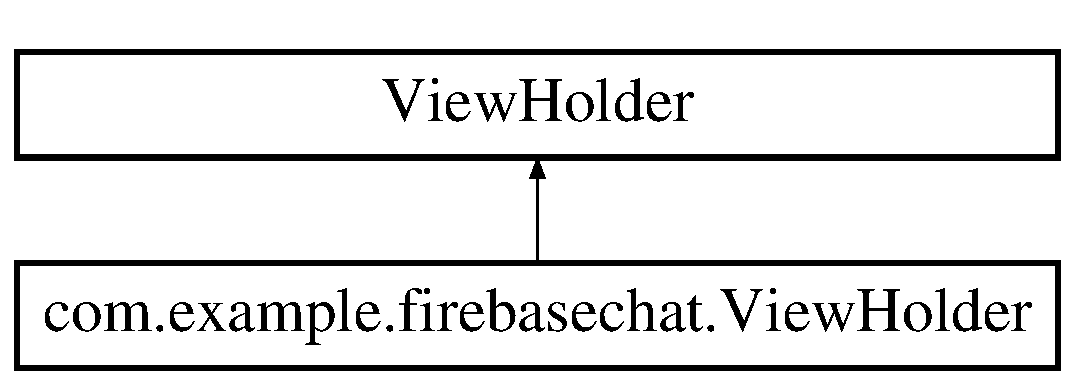
\includegraphics[height=2.000000cm]{classcom_1_1example_1_1firebasechat_1_1_view_holder}
\end{center}
\end{figure}
\subsection*{Открытые члены}
\begin{DoxyCompactItemize}
\item 
\mbox{\hyperlink{classcom_1_1example_1_1firebasechat_1_1_view_holder_a6659514a237d574a53725eead8789579}{View\+Holder}} (View Item\+View)
\end{DoxyCompactItemize}


\subsection{Подробное описание}
Класс holder отображения сообщений в Recycler\+View. 

См. определение в файле View\+Holder.\+java строка 10



\subsection{Конструктор(ы)}
\mbox{\Hypertarget{classcom_1_1example_1_1firebasechat_1_1_view_holder_a6659514a237d574a53725eead8789579}\label{classcom_1_1example_1_1firebasechat_1_1_view_holder_a6659514a237d574a53725eead8789579}} 
\index{com\+::example\+::firebasechat\+::\+View\+Holder@{com\+::example\+::firebasechat\+::\+View\+Holder}!View\+Holder@{View\+Holder}}
\index{View\+Holder@{View\+Holder}!com\+::example\+::firebasechat\+::\+View\+Holder@{com\+::example\+::firebasechat\+::\+View\+Holder}}
\subsubsection{\texorpdfstring{View\+Holder()}{ViewHolder()}}
{\footnotesize\ttfamily com.\+example.\+firebasechat.\+View\+Holder.\+View\+Holder (\begin{DoxyParamCaption}\item[{View}]{Item\+View }\end{DoxyParamCaption})}



См. определение в файле View\+Holder.\+java строка 14



Объявления и описания членов класса находятся в файле\+:\begin{DoxyCompactItemize}
\item 
C\+:/\+Games/\+Back\+Up/\+Fire\+Basechat/app/src/main/java/com/example/firebasechat/\mbox{\hyperlink{_view_holder_8java}{View\+Holder.\+java}}\end{DoxyCompactItemize}

\chapter{Файлы}
\hypertarget{_authors_8java}{}\section{Файл C\+:/\+Games/\+Back\+Up/\+Fire\+Basechat/app/src/main/java/com/example/firebasechat/\+Authors.java}
\label{_authors_8java}\index{C\+:/\+Games/\+Back\+Up/\+Fire\+Basechat/app/src/main/java/com/example/firebasechat/\+Authors.\+java@{C\+:/\+Games/\+Back\+Up/\+Fire\+Basechat/app/src/main/java/com/example/firebasechat/\+Authors.\+java}}
\subsection*{Классы}
\begin{DoxyCompactItemize}
\item 
class \mbox{\hyperlink{classcom_1_1example_1_1firebasechat_1_1_authors}{com.\+example.\+firebasechat.\+Authors}}
\begin{DoxyCompactList}\small\item\em Класс для отображения страницы с информацией о создателях \end{DoxyCompactList}\end{DoxyCompactItemize}
\subsection*{Пакеты}
\begin{DoxyCompactItemize}
\item 
package \mbox{\hyperlink{namespacecom_1_1example_1_1firebasechat}{com.\+example.\+firebasechat}}
\end{DoxyCompactItemize}

\hypertarget{_chat_room_8java}{}\section{Файл C\+:/\+Games/\+Back\+Up/\+Fire\+Basechat/app/src/main/java/com/example/firebasechat/\+Chat\+Room.java}
\label{_chat_room_8java}\index{C\+:/\+Games/\+Back\+Up/\+Fire\+Basechat/app/src/main/java/com/example/firebasechat/\+Chat\+Room.\+java@{C\+:/\+Games/\+Back\+Up/\+Fire\+Basechat/app/src/main/java/com/example/firebasechat/\+Chat\+Room.\+java}}
\subsection*{Классы}
\begin{DoxyCompactItemize}
\item 
class \mbox{\hyperlink{classcom_1_1example_1_1firebasechat_1_1_chat_room}{com.\+example.\+firebasechat.\+Chat\+Room}}
\begin{DoxyCompactList}\small\item\em Данное Activity представляет собой комнату обмена зашифрованными сообщениями \end{DoxyCompactList}\end{DoxyCompactItemize}
\subsection*{Пакеты}
\begin{DoxyCompactItemize}
\item 
package \mbox{\hyperlink{namespacecom_1_1example_1_1firebasechat}{com.\+example.\+firebasechat}}
\end{DoxyCompactItemize}

\hypertarget{_main_activity_8java}{}\section{Файл C\+:/\+Games/\+Back\+Up/\+Fire\+Basechat/app/src/main/java/com/example/firebasechat/\+Main\+Activity.java}
\label{_main_activity_8java}\index{C\+:/\+Games/\+Back\+Up/\+Fire\+Basechat/app/src/main/java/com/example/firebasechat/\+Main\+Activity.\+java@{C\+:/\+Games/\+Back\+Up/\+Fire\+Basechat/app/src/main/java/com/example/firebasechat/\+Main\+Activity.\+java}}
\subsection*{Классы}
\begin{DoxyCompactItemize}
\item 
class \mbox{\hyperlink{classcom_1_1example_1_1firebasechat_1_1_main_activity}{com.\+example.\+firebasechat.\+Main\+Activity}}
\begin{DoxyCompactList}\small\item\em Activity регистрации и авторизации пользователей \end{DoxyCompactList}\item 
class \mbox{\hyperlink{classcom_1_1example_1_1firebasechat_1_1_main_activity_1_1_key___thread}{com.\+example.\+firebasechat.\+Main\+Activity.\+Key\+\_\+\+Thread}}
\begin{DoxyCompactList}\small\item\em Поток для обработки генерации ключей \end{DoxyCompactList}\end{DoxyCompactItemize}
\subsection*{Пакеты}
\begin{DoxyCompactItemize}
\item 
package \mbox{\hyperlink{namespacecom_1_1example_1_1firebasechat}{com.\+example.\+firebasechat}}
\end{DoxyCompactItemize}

\hypertarget{_message_8java}{}\section{Файл C\+:/\+Games/\+Back\+Up/\+Fire\+Basechat/app/src/main/java/com/example/firebasechat/\+Message.java}
\label{_message_8java}\index{C\+:/\+Games/\+Back\+Up/\+Fire\+Basechat/app/src/main/java/com/example/firebasechat/\+Message.\+java@{C\+:/\+Games/\+Back\+Up/\+Fire\+Basechat/app/src/main/java/com/example/firebasechat/\+Message.\+java}}
\subsection*{Классы}
\begin{DoxyCompactItemize}
\item 
class \mbox{\hyperlink{classcom_1_1example_1_1firebasechat_1_1_message}{com.\+example.\+firebasechat.\+Message}}
\begin{DoxyCompactList}\small\item\em Класс сообщений пользователей \end{DoxyCompactList}\end{DoxyCompactItemize}
\subsection*{Пакеты}
\begin{DoxyCompactItemize}
\item 
package \mbox{\hyperlink{namespacecom_1_1example_1_1firebasechat}{com.\+example.\+firebasechat}}
\end{DoxyCompactItemize}

\hypertarget{_splash_activity_8java}{}\section{Файл C\+:/\+Games/\+Back\+Up/\+Fire\+Basechat/app/src/main/java/com/example/firebasechat/\+Splash\+Activity.java}
\label{_splash_activity_8java}\index{C\+:/\+Games/\+Back\+Up/\+Fire\+Basechat/app/src/main/java/com/example/firebasechat/\+Splash\+Activity.\+java@{C\+:/\+Games/\+Back\+Up/\+Fire\+Basechat/app/src/main/java/com/example/firebasechat/\+Splash\+Activity.\+java}}
\subsection*{Классы}
\begin{DoxyCompactItemize}
\item 
class \mbox{\hyperlink{classcom_1_1example_1_1firebasechat_1_1_splash_activity}{com.\+example.\+firebasechat.\+Splash\+Activity}}
\begin{DoxyCompactList}\small\item\em Заставка приложения \end{DoxyCompactList}\end{DoxyCompactItemize}
\subsection*{Пакеты}
\begin{DoxyCompactItemize}
\item 
package \mbox{\hyperlink{namespacecom_1_1example_1_1firebasechat}{com.\+example.\+firebasechat}}
\end{DoxyCompactItemize}

\hypertarget{_user_8java}{}\section{Файл C\+:/\+Games/\+Back\+Up/\+Fire\+Basechat/app/src/main/java/com/example/firebasechat/\+User.java}
\label{_user_8java}\index{C\+:/\+Games/\+Back\+Up/\+Fire\+Basechat/app/src/main/java/com/example/firebasechat/\+User.\+java@{C\+:/\+Games/\+Back\+Up/\+Fire\+Basechat/app/src/main/java/com/example/firebasechat/\+User.\+java}}
\subsection*{Классы}
\begin{DoxyCompactItemize}
\item 
class \mbox{\hyperlink{classcom_1_1example_1_1firebasechat_1_1_user}{com.\+example.\+firebasechat.\+User}}
\begin{DoxyCompactList}\small\item\em Класс пользователя \end{DoxyCompactList}\end{DoxyCompactItemize}
\subsection*{Пакеты}
\begin{DoxyCompactItemize}
\item 
package \mbox{\hyperlink{namespacecom_1_1example_1_1firebasechat}{com.\+example.\+firebasechat}}
\end{DoxyCompactItemize}

\hypertarget{_view_holder_8java}{}\section{Файл C\+:/\+Games/\+Back\+Up/\+Fire\+Basechat/app/src/main/java/com/example/firebasechat/\+View\+Holder.java}
\label{_view_holder_8java}\index{C\+:/\+Games/\+Back\+Up/\+Fire\+Basechat/app/src/main/java/com/example/firebasechat/\+View\+Holder.\+java@{C\+:/\+Games/\+Back\+Up/\+Fire\+Basechat/app/src/main/java/com/example/firebasechat/\+View\+Holder.\+java}}
\subsection*{Классы}
\begin{DoxyCompactItemize}
\item 
class \mbox{\hyperlink{classcom_1_1example_1_1firebasechat_1_1_view_holder}{com.\+example.\+firebasechat.\+View\+Holder}}
\begin{DoxyCompactList}\small\item\em Класс holder отображения сообщений в Recycler\+View. \end{DoxyCompactList}\end{DoxyCompactItemize}
\subsection*{Пакеты}
\begin{DoxyCompactItemize}
\item 
package \mbox{\hyperlink{namespacecom_1_1example_1_1firebasechat}{com.\+example.\+firebasechat}}
\end{DoxyCompactItemize}

%--- End generated contents ---

% Index
\backmatter
\newpage
\phantomsection
\clearemptydoublepage
\addcontentsline{toc}{chapter}{Алфавитный указатель}
\printindex

\end{document}
